% !TEX encoding = UTF-8
% !TEX program = pdflatex
% !TEX spellcheck = it_IT

\documentclass[a4paper, 11pt]{article}

% appendix

\usepackage[toc,page]{appendix}

% sintassi
\usepackage[T1]{fontenc}
\usepackage[utf8]{inputenc}
\usepackage[english]{babel}
\DeclareUnicodeCharacter{00A0}{~}
\usepackage{fullpage}
%\usepackage[cochineal]{newtxmath}
%\usepackage{crimson,verbatim}
\usepackage{textcomp}
\usepackage{color,soul,hyperref,mwe}

% matematica e chimica

\usepackage{siunitx,amsmath,bm,chemfig}
\newcommand{\ud}{\mathop{}\!\mathrm{d}}
\sisetup{detect-all,math-rm = \ensuremath}
%\usepackage{arev}
\usepackage[charter]{mathdesign}


\setatomsep{2em}

\newcommand\setpolymerdelim[2]{\def\delimleft{#1}\def\delimright{#2}} 
\def\makebraces[#1,#2]#3#4#5{% 
\edef\delimhalfdim{\the\dimexpr(#1+#2)/2}% 
\edef\delimvshift{\the\dimexpr(#1-#2)/2}% 
\chemmove{% 
\node[at=(#4),yshift=(\delimvshift)] {$\left\delimleft\vrule height\delimhalfdim depth\delimhalfdim 
width0pt\right.$};% 
\node[at=(#5),yshift=(\delimvshift)] 
{$\left.\vrule height\delimhalfdim depth\delimhalfdim 
width0pt\right\delimright_{\rlap{$\scriptstyle#3$}}$};}} 
\setpolymerdelim()

% tabelle e grafica
\usepackage{booktabs,graphicx,graphbox,subfig,caption,pdfpages}
\captionsetup{font=small,
	format=hang,
	justification=centering,
	singlelinecheck=true,
	labelfont={sf,bf}	
}
\usepackage{float}
\floatstyle{plaintop}
\restylefloat{table}
\usepackage{multirow}
\usepackage{fancyhdr}
\pagestyle{fancy}
\fancyhead[LE,RO]{\textsl{\rightmark}}
\fancyhead[LO,RE]{\nouppercase{\leftmark}}
\fancyfoot[C]{\thepage}
\usepackage[margin=1in,headsep=.3in]{geometry}
\usepackage[suftesi]{frontespizio}
\usepackage{xparse}
\setlength\parindent{0pt}

\newenvironment{chapterabstract}{%
  \par\nobreak\noindent
  \textbf{\textit{Abstract}\hrulefill}\nobreak
  %\small
  \noindent\ignorespaces
}{%
  \par\nobreak\normalsize
  \vskip-\ht\strutbox\noindent
  \textbf{\hrulefill}%
}
\makeatletter
\NewDocumentCommand\headerspdf{ O {pages=-} m }{% [options for include pdf]{filename.pdf}
  \includepdf[%
    #1,
    pagecommand={\thispagestyle{fancy}},
    scale=1,
    ]{#2}}
\NewDocumentCommand\secpdf{somO{1}m}{% [short title]{section title}[page specification]{filename.pdf} --- possibly starred
  \clearpage
  \thispagestyle{fancy}%
  \includepdf[%
    pages=#4,
    pagecommand={%
      \IfBooleanTF{#1}{%
        \section*{#3}}{%
        \IfNoValueTF{#2}{%
          \section{#3}}{%
          \section[#2]{#3}}}},
    scale=.65,
    ]%
    {#5}}
\makeatother

\begin{document}

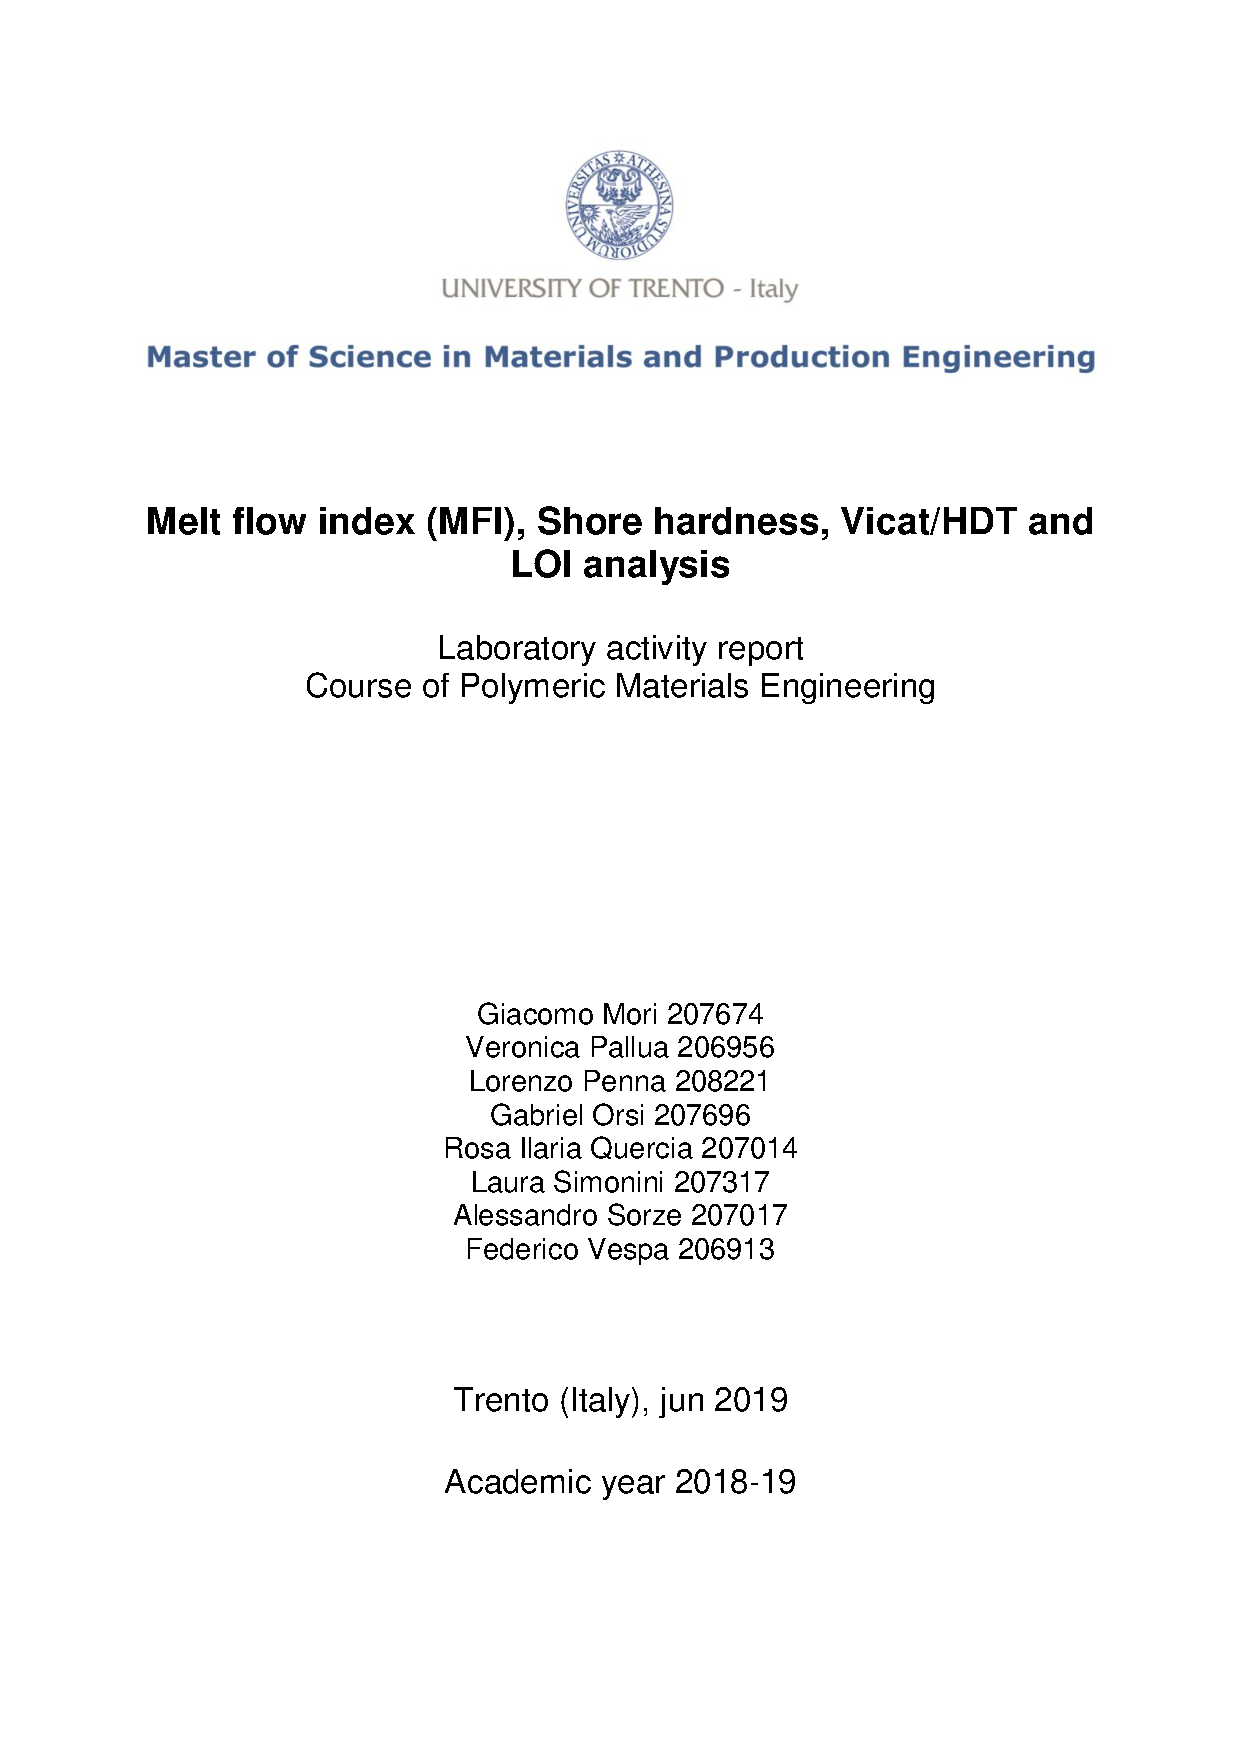
\includepdf[pages=-]{frontespizio3.pdf}

\begin{chapterabstract}

Different polymer properties were evaluated by performing Vicat test, melt flow index (MFI) analysis, Shore hardness and limiting oxygen flammability (LOI).
Vicat test was used to estimate the deformability of three polymers: polycarbonate (PC), acrylonitrile butadiene styrene (ABS) and polypropylene (PP). Since PS and ABS are amorphous polymers, the Vicat temperatures do not change with the load, while for PP, which is a semi crystalline polymer, Vicat temperature varies with the load.
With MFI analyses some rheological reckonings are possible. First, the MFI increases exponentially with temperature and the applied load; moreover, by testing three different polypropylenes, increasing the MFI, the molecular weight (MW) decreases exponentially. The phenomenon of die swelling also depends on MW: for higher molecular weight, the die swell is lower due to high possibility of orientation of longer chains. The results of MFI calculations were also used to evaluate the activation energy ($E_a$) of viscous flow; for PPH 7089 the average $E_a$ is about 50 kJ/mol.
Shore hardness test was used to measure the hardness of different polymers. It was found that the Shore A test is suitable for the softer materials while Shore D is suitable for the harder ones. It is interesting to notice that polyurethane (PU), which is a thermoset polymer, shows a wide range of hardness (Shore A) from 50 to 95.
Limiting oxygen index was used to investigate the relative flammability of four polymers i.e. polyethylene (PE), PP, PC and ABS. PC has the higher LOI (33\%) resulting less flammable than the others.

\end{chapterabstract} 

\section{Introduction}

The aim of this laboratory session is to study rheological properties of different polymeric materials, together with thermal evolution of stiffness (Vicat), measurement of hardness (Shore A and D) and flammability (limit oxygen index, LOI). 

\subsection {Polymers and products}

A wide selection of polymeric materials has been studied, particularly for hardness measurements, including either thermoplastics and thermosets, semicrystalline and amorphous polymers. In Figure \ref{fig:rubber} samples for hardness measurement are displayed. 
\begin{figure}[h!]
	\centering
	{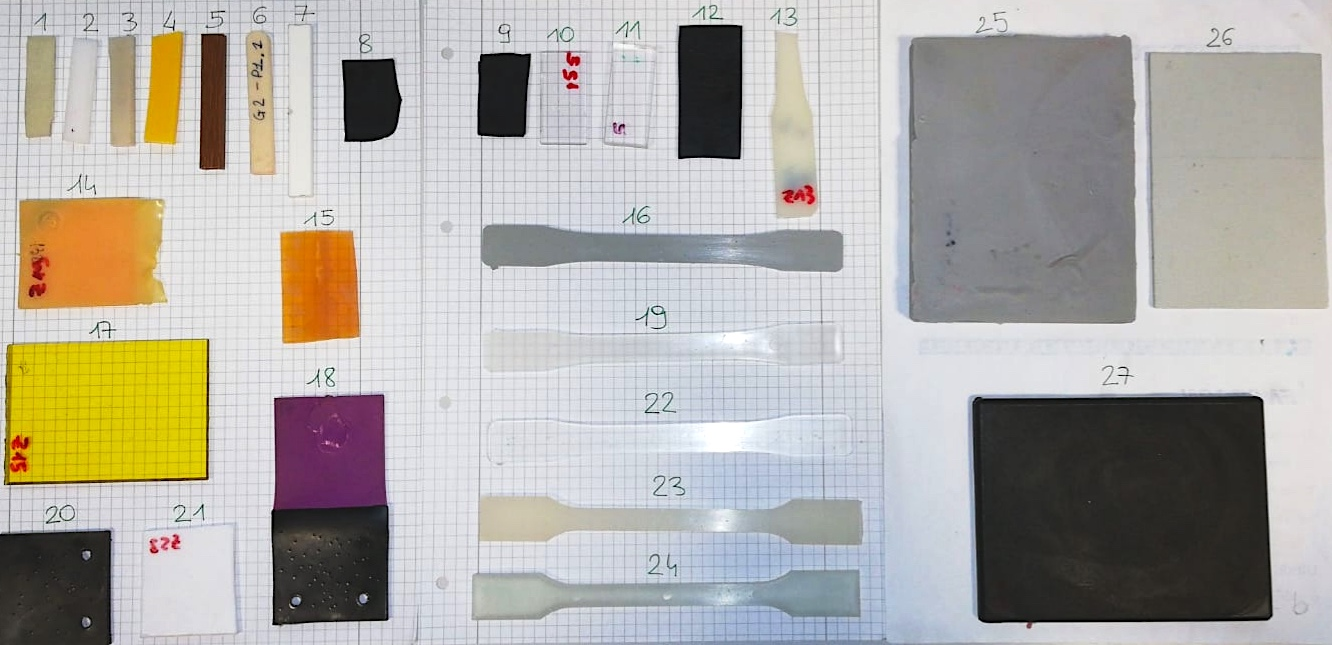
\includegraphics[scale=0.3]{rubber}}
	\captionsetup{justification=centering}
	\caption{Samples for hardness measurements.}
	\label{fig:rubber}
\end{figure}
\newpage
Polypropylene has been deeply studied in its rheological properties, highlighting common properties like activation energy of viscous flow and die swelling. In Figure \ref{fig:melt} extrudates of polystyrene and polypropylene from melt flow index analysis are displayed. 
\begin{figure}[h!]
	\centering
	{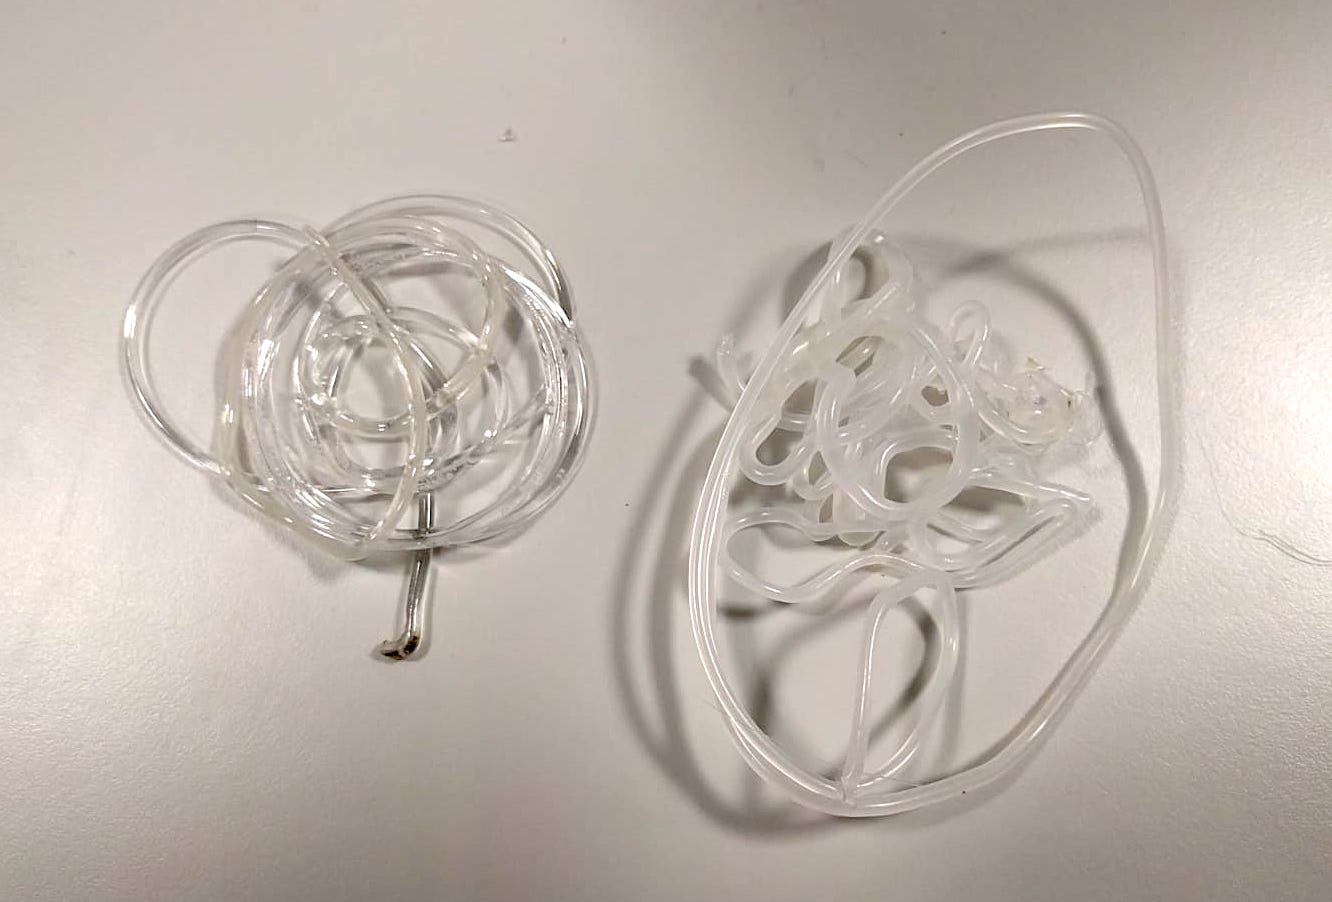
\includegraphics[scale=0.2]{melt}}
	\captionsetup{justification=centering}
	\caption{Extrudates of polystyrene (left) and polypropylene (right) from melt flow index analysis.}
	\label{fig:melt}
\end{figure}\\
Vicat analysis has been done on ready made samples of polycarbonate (PC), acrylonitrile-butadiene-styrene copolymer (ABS) and polypropylene (PP). In Figure \ref{fig:chem} chemical formulas of these polymers are reported. 
\begin{figure}[h!]
	\centering
	\subfloat[][]
	{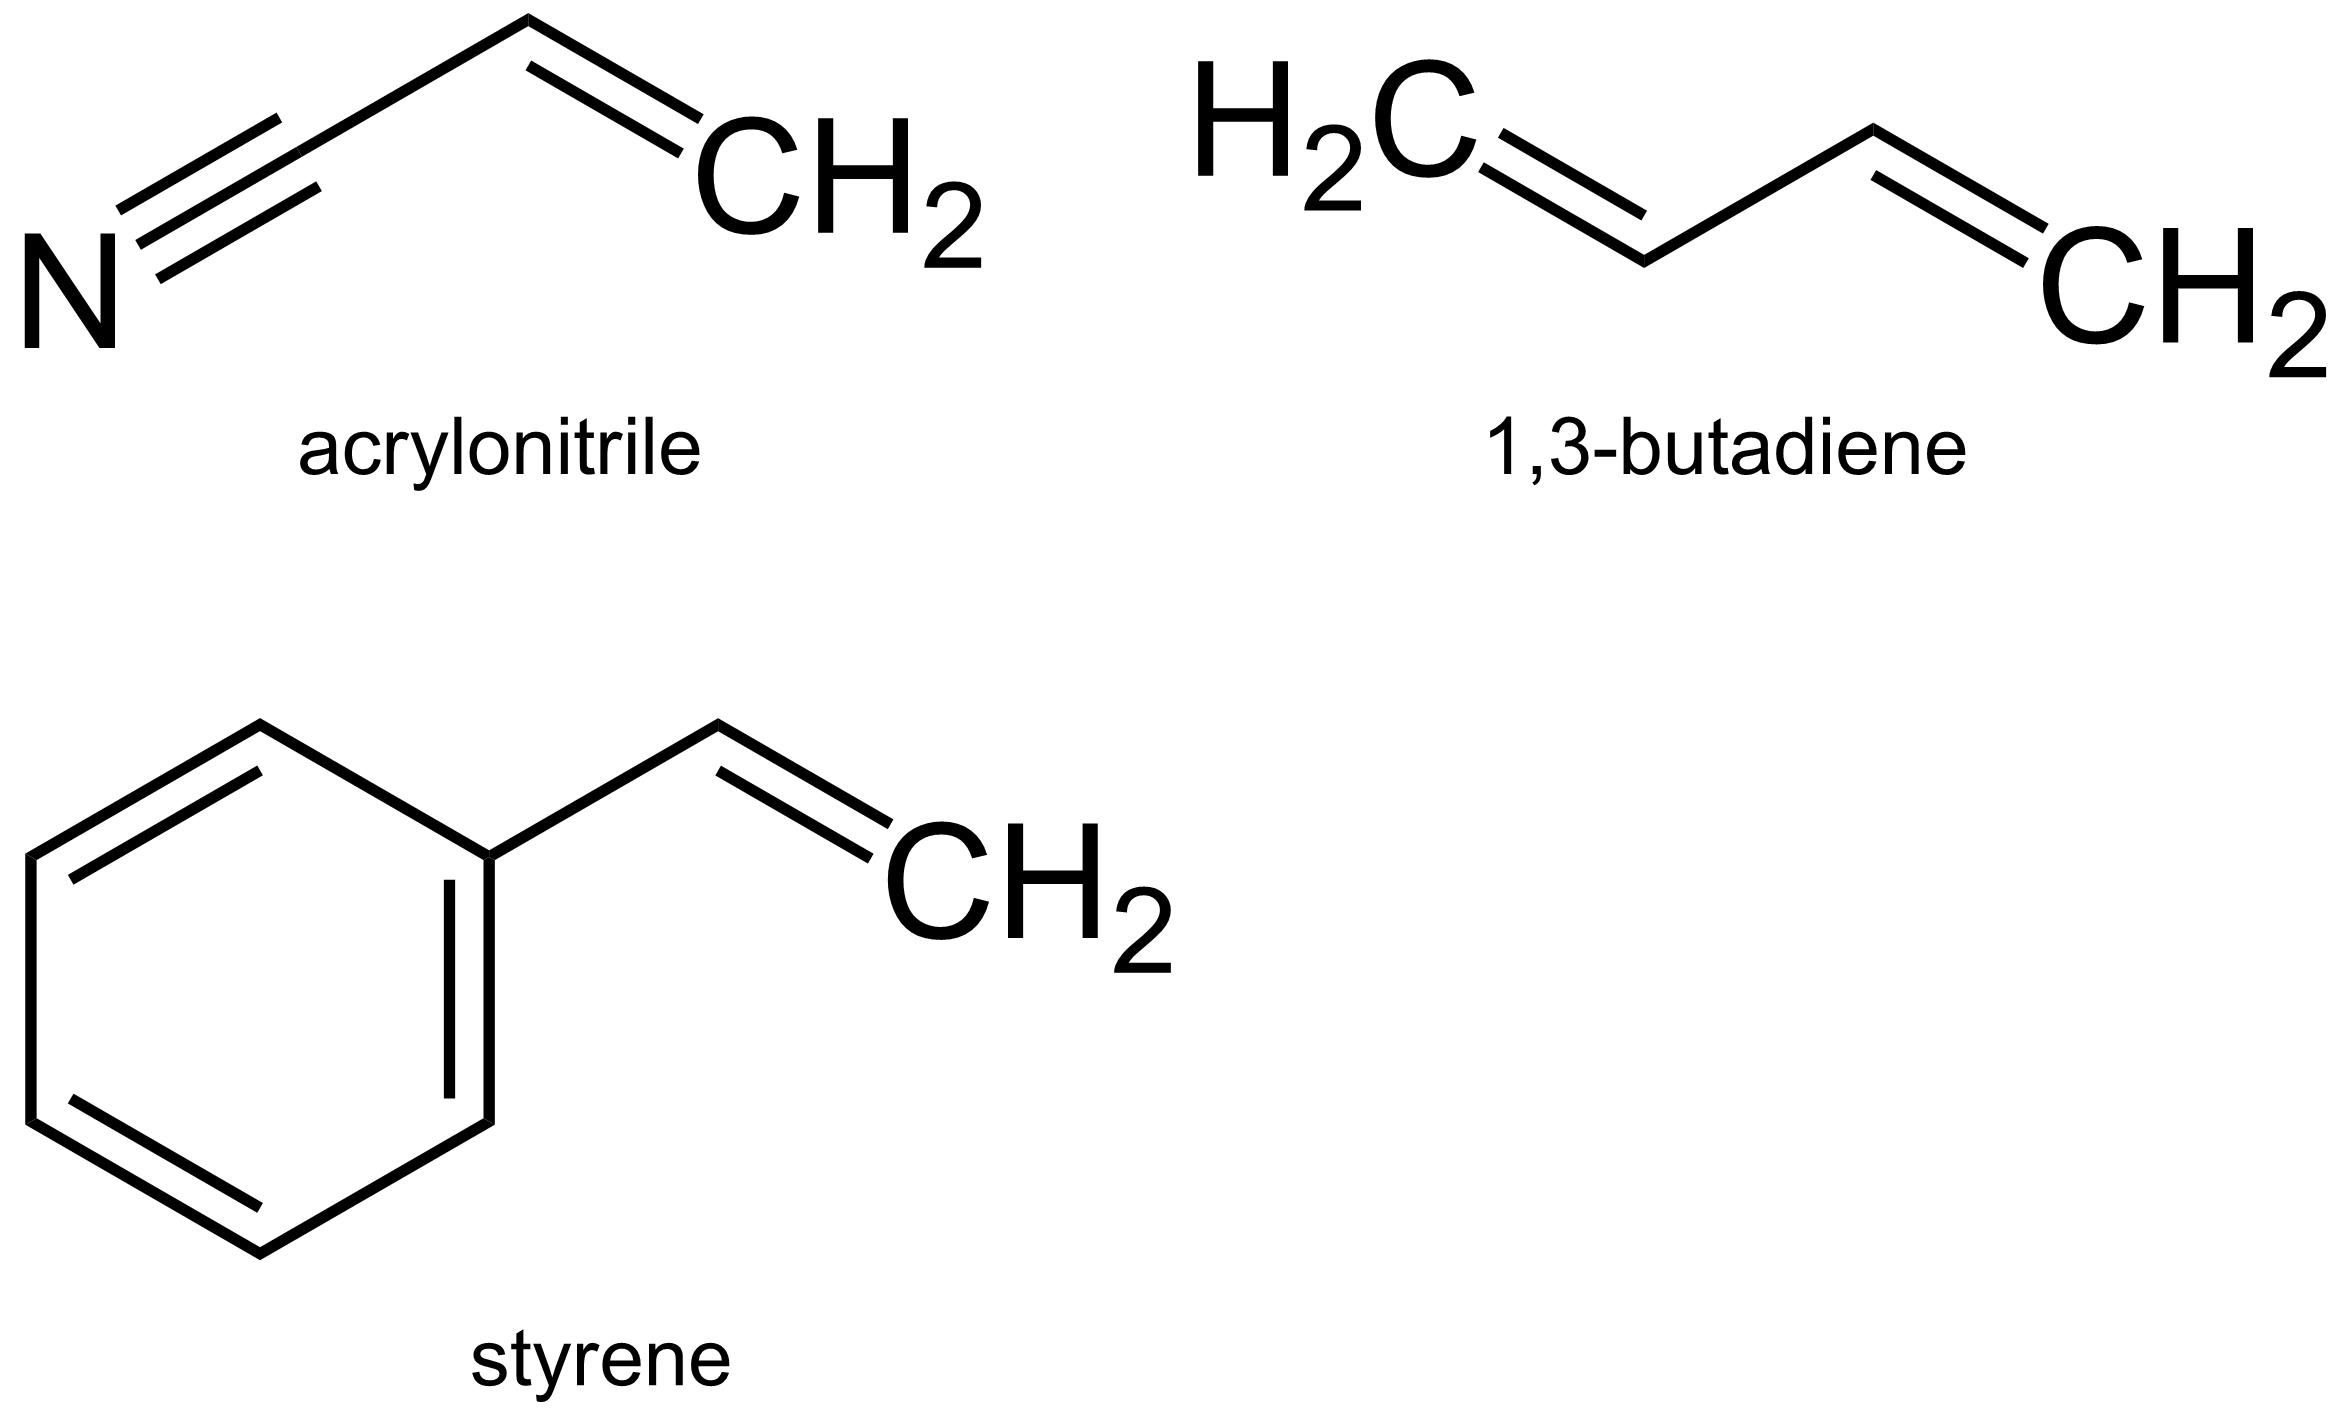
\includegraphics[align=c,scale=0.07]{abs}} \quad 
	\subfloat[][]
	{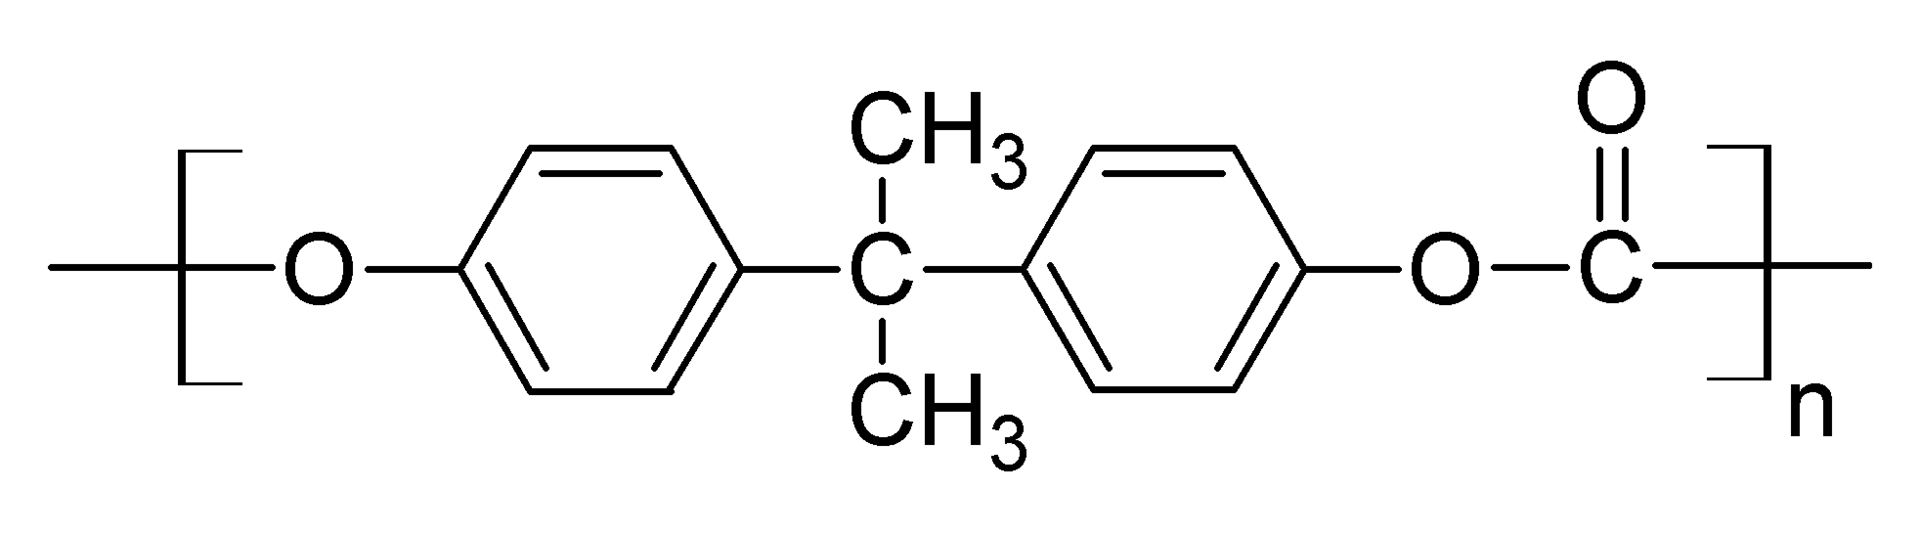
\includegraphics[align=c,scale=0.9]{PC}} \quad
	\subfloat[][]
	{
\includegraphics[align=c,scale=0.08]{pp}}  
	\captionsetup{justification=centering}
	\caption{Chemical formulas of (a) ABS (three constituents), (b) PC and (c) PP.}
	\label{fig:chem}
\end{figure}\\
LOI measurements have been one on samples of polyethylene (PE), PP, PC and ABS. In Figure \ref{fig:LOI} samples after the experimental activity are displayed. 
\begin{figure}[h!]
	\centering
	{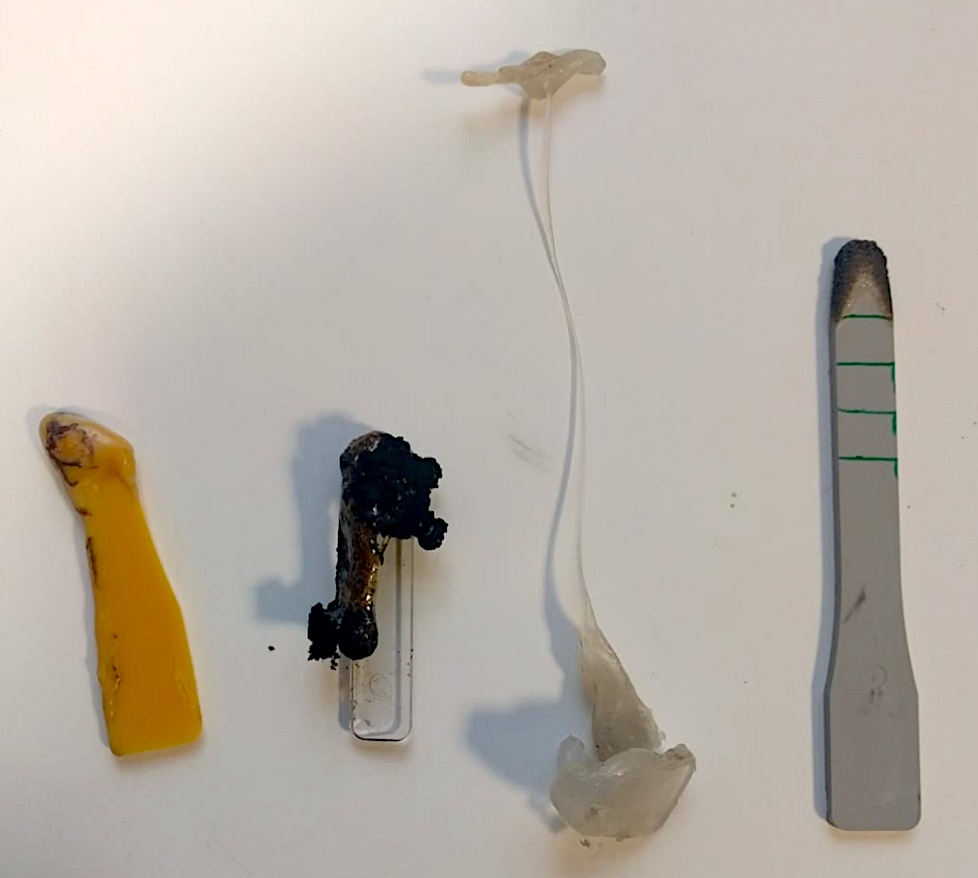
\includegraphics[scale=0.2]{LOI}}
	\captionsetup{justification=centering}
	\caption{From left to right: PE, PC, PP and ABS samples after the experimental activity.}
	\label{fig:LOI}
\end{figure}\\

\section{Materials and methods}

\subsection{Materials}

Different polymeric samples have been provided by University of Trento to get Vicat analysis: PC, ABS and PP. A long list of samples have been tested in Shore analysis, as reported in Table \ref{tab:polymers}, where TP = termoplastic, TS = thermoset and E = elastomer.

\begin{table}[htp]
	\centering
	$
	\begin{array}{ccc}
	\toprule
	\textbf{number} & \textbf{sample} & \textbf{type} \\
	\midrule
	1,24 & \text{PP + GF} & \text{TP}\\
	2 & \text{POM} & \text{TP}\\
	3 & \text{PA 11} & \text{TP}\\
	4 & \text{PE} & \text{TP}\\
	5 & \text{PVC} & \text{TP}\\
	6 & \text{PMMA + BaSO} & \text{TP}\\
	7 & \text{PBT} & \text{TP}\\
	8,9 & \text{EPDM} & \text{E}\\
    10 & \text{PC} & \text{TP}\\
	11 & \text{PMMA} & \text{TP}\\
	12 & \text{generic rubber} & \text{E}\\
	13 & \text{PA 6} & \text{TP}\\
	14,18,20,25,27 & \text{PU} & \text{TS}\\
	15 & \text{Silicone} & \text{E}\\
	16 & \text{ABS} & \text{TP}\\
	17 & \text{SAN} & \text{TP}\\
	19 & \text{PP} & \text{TP}\\
	21 & \text{PTFE} & \text{TP}\\
	22 & \text{COC} & \text{TP}\\
	23 & \text{PA} & \text{TP}\\
	26 & \text{PET} & \text{TP}\\
	\bottomrule
	\end{array}
	$
	\caption{Materials used in Shore analyses.}
	\label{tab:polymers}
\end{table}
Three different polypropylene samples have been provided by different companies in order to carry out melt flow index analyses, as reported in Table \ref{tab:PP}. 
\begin{table}[htp]
	\centering
	$
	\begin{array}{llc}
	\toprule
	\textbf{Sample} & \textbf{Product name} & \textbf{Typical MFI} \, \text{(g/10min)}  \\
	& & (230^\circ \text{C, 2.16 kg}) \\
	\midrule
	\text{PP–1} & \text{PPH 7089} & 12\\
	\text{PP–2} & \text{Moplen HP 500 N} & 5\\
	\text{PP–3} & \text{Borealis} & 25\\
	\bottomrule
	\end{array}
	$
	\caption{Polypropylene materials used.}
	\label{tab:PP}
\end{table}
\\
For limit oxygen index analyses tested samples are PE, PP, PC and ABS plastics provided by University of Trento. 

\subsection{Sample preparation}

Samples have been prepared in function of the specific experimental activities. Vicat samples were ready made in the right geometry for the analysis. Shore samples were ready made too, ready for the analysis as provided. Melt flow index samples are polymer granules as provided, that have been fed into the insturment for the analysis without any further processing of them. 

\subsubsection{Manual drawing for x-ray diffraction (XRD) and mechanical testing}

An amount of granules for melt flow index analysis has been used in order to manually draw fibers of polypropylene. The polymeric melt flowing out of the instrument has been stretched manually, imposing a moderate strength, with the purpose of obtaining fibers, that will be used for x-ray diffraction analyses and mechanical tensile testings.  

\section{Experimental activity}

\subsection{Vicat Softening Temperature analysis (VST)}

The test has been carried out in two configurations, with instrument Vicat Tester MP/3 and according to the normative ASTM~\cite{VICAT}:

\begin{itemize}

\item $120^\circ$C/h, 10 N;

\item $120^\circ$C/h, 50 N.

\end{itemize}
Polymers analyzed are: PC, ABS and PP. Samples dimensions are $1\times1$ cm and the thickness is 3.2 mm which is higher than the maximum penetration depth. Vicat temperarature is the temperature at which the penetration is about 1 mm: $T_\text{vicat}^\text{10}$ is obtained with a load of 10 N while $T_\text{vicat}^\text{50}$ is obtained with a load of 50 N. 

\subsection{Melt flow index (MFI) measurement}

Melt flow index (MFI) analysis has been carried out with a Dynisco Melt Flow Indexer. According to ASTM standard, the typical test conditions for PP are temperature of $230 ^\circ$C and load of $2.16\  \text{kg}$. \\
A first analysis has been conducted on PP–1 with 9 different configurations changing the temperature ($190 ^\circ$C, $210 ^\circ$C, $230 ^\circ$C) and changing the load ($2.16\ \text{kg}, 5.0\ \text{kg}, 7.06 \ \text{kg}$). \\
A second analysis has been done on PP–2 at $230 ^\circ$C under loads of  $2.16\ \text{kg}$ and  $7.06\ \text{kg}$. \\
A third analysis has been carried out on PP–3 at $230 ^\circ$C under $2.16\ \text{kg}$. \\
For each configuration six samples have been produced. The first one has been used for the evaluation of die swelling according to Equation \ref{eq:die}:
\begin{equation}
\text{Die\ swell} = \bigg(\frac{D_\text{ex}}{D_\text{or}}\bigg)^2
\label{eq:die}
\end{equation}
where $D_\text{ex}$ is the measured diameter of extrudate and $D_\text{or}$ is the diameter of the orifice (die) defined by ASTM standard~\cite{MFI}. \\
The MFI has been calculated by Equation \ref{eq:mfi}: 
\begin{equation}
\text{MFI} = \frac{m_\text{ex}}{t}
\label{eq:mfi}
\end{equation}
where $m_\text{ex}$ is the weight of the extrudate and $t$ is the extrusion time. According to standard the unit of measure of MFI is $\text{g/10min}$ standard. For sake of semplicity, the measurements have been taken in lower times and then reported scaled to 10 minutes. 

\subsubsection{Molecular weight calculation}
From reference handbook~\cite{handbook} specific values of MFI in function of molecular weight (reported in Table \ref{tab:mw}) have been used for built a curve that permits to estimate the molecular weight of each type of PP knowing the melt flow index. For this calculation MFI of ASTM standard~\cite{MFI} has been taken into account.
\begin{table}[htp]
	\centering
	$
	\begin{array}{cc}
	\toprule
	\textbf{Molecular Weight} \, \text{(g/mol)} & \textbf{Melt Flow Index} \, \text{(g/10min)} \\
	\text{MW}\cdot 10^{-3} & (230^\circ \text{C, 2.16 kg}) \\
	\midrule
	 142 & 22.8 \\
	 180 & 7.3 \\
	 220 & 3.5 \\
	 292 & 1.2 \\
	 358 & 0.39 \\
	\bottomrule
	\end{array}
	$
	\caption{MFI in function of molecular weight of PP according to literature~\cite{handbook} .}
	\label{tab:mw}
\end{table}

\subsubsection{Activation energy calculation}
From melt flow index values it can be evaluated the activation energy using Arrhenius model described by Equation \ref{eq:arr}
\begin{equation}
\text{MFI} = A e ^{-\frac{E_a}{RT}}
\label{eq:arr}
\end{equation}
where $A$ is a constant, $E_a$ is activation energy, $T$ is the process temperature  (in K) and $R$ is the gas constant. This calculation has been done for each applied load. Linearizing the Equation \ref{eq:arr} through logaritm properties the activation energy can be expressed as the slope of the curve.

\subsection{Shore hardness measurement}

Shore hardness scales are used to compare the behaviour of different materials under load. The durometer ATS FAAR has been used.
Two different scales have been employed:
\begin{itemize}
\item Shore A: presents a conical indentor and the weight applied is about 0.488 Kg. It is used for soft and flexible materials;
\item Shore D: presents a sharp indentor and the weight applied is about 3.964 Kg. It is used for hard and semi-rigid materials.

\end{itemize}

Different polymeric specimens have been tested: for each, three mesurements has been carried out with a waiting time of three seconds. Analyzed polymers are reported in the previous Table \ref{tab:polymers}.

\subsection{Limit oxygen index (LOI) measurement}

Analyzed polymers are PE, PP, PC and ABS, with instrument Ceast Oxygen Index. This test allows to predict the behaviour of polymers when they are exposed to the flame. Air is blowed in the working column and the amount of oxygen is carefully modulated (its value has been taken around 21\%). Specimens are exposed to the flame for three minutes, accordingly to standard procedure by ASTM~\cite{LOI}. In Table \ref{tab:oxygen} the percentage of oxygen used are reported
\begin{table}[htp]
	\centering
	$
	\begin{array}{cc}
	\toprule
	\textbf{Sample} & \textbf{Oxygen ($\%$)}\\
	\midrule
	\textbf{PE} & 20 \\
	\textbf{PP} & 22\\
	\textbf{PC} & 33 \\
	\textbf{ABS} & 20\\
	\bottomrule
	\end{array}
	$
	\caption{Percentage of oxygen used in LOI measurements.}
	\label{tab:oxygen}
\end{table}

\newpage

\section{Results and discussion}

\subsection{Vicat analysis (VST)}

The results of the penetration test are reported in the following Figures \ref{fig:vicat}a-b.

\begin{figure}[htp]
	\centering
	\subfloat[][]
	{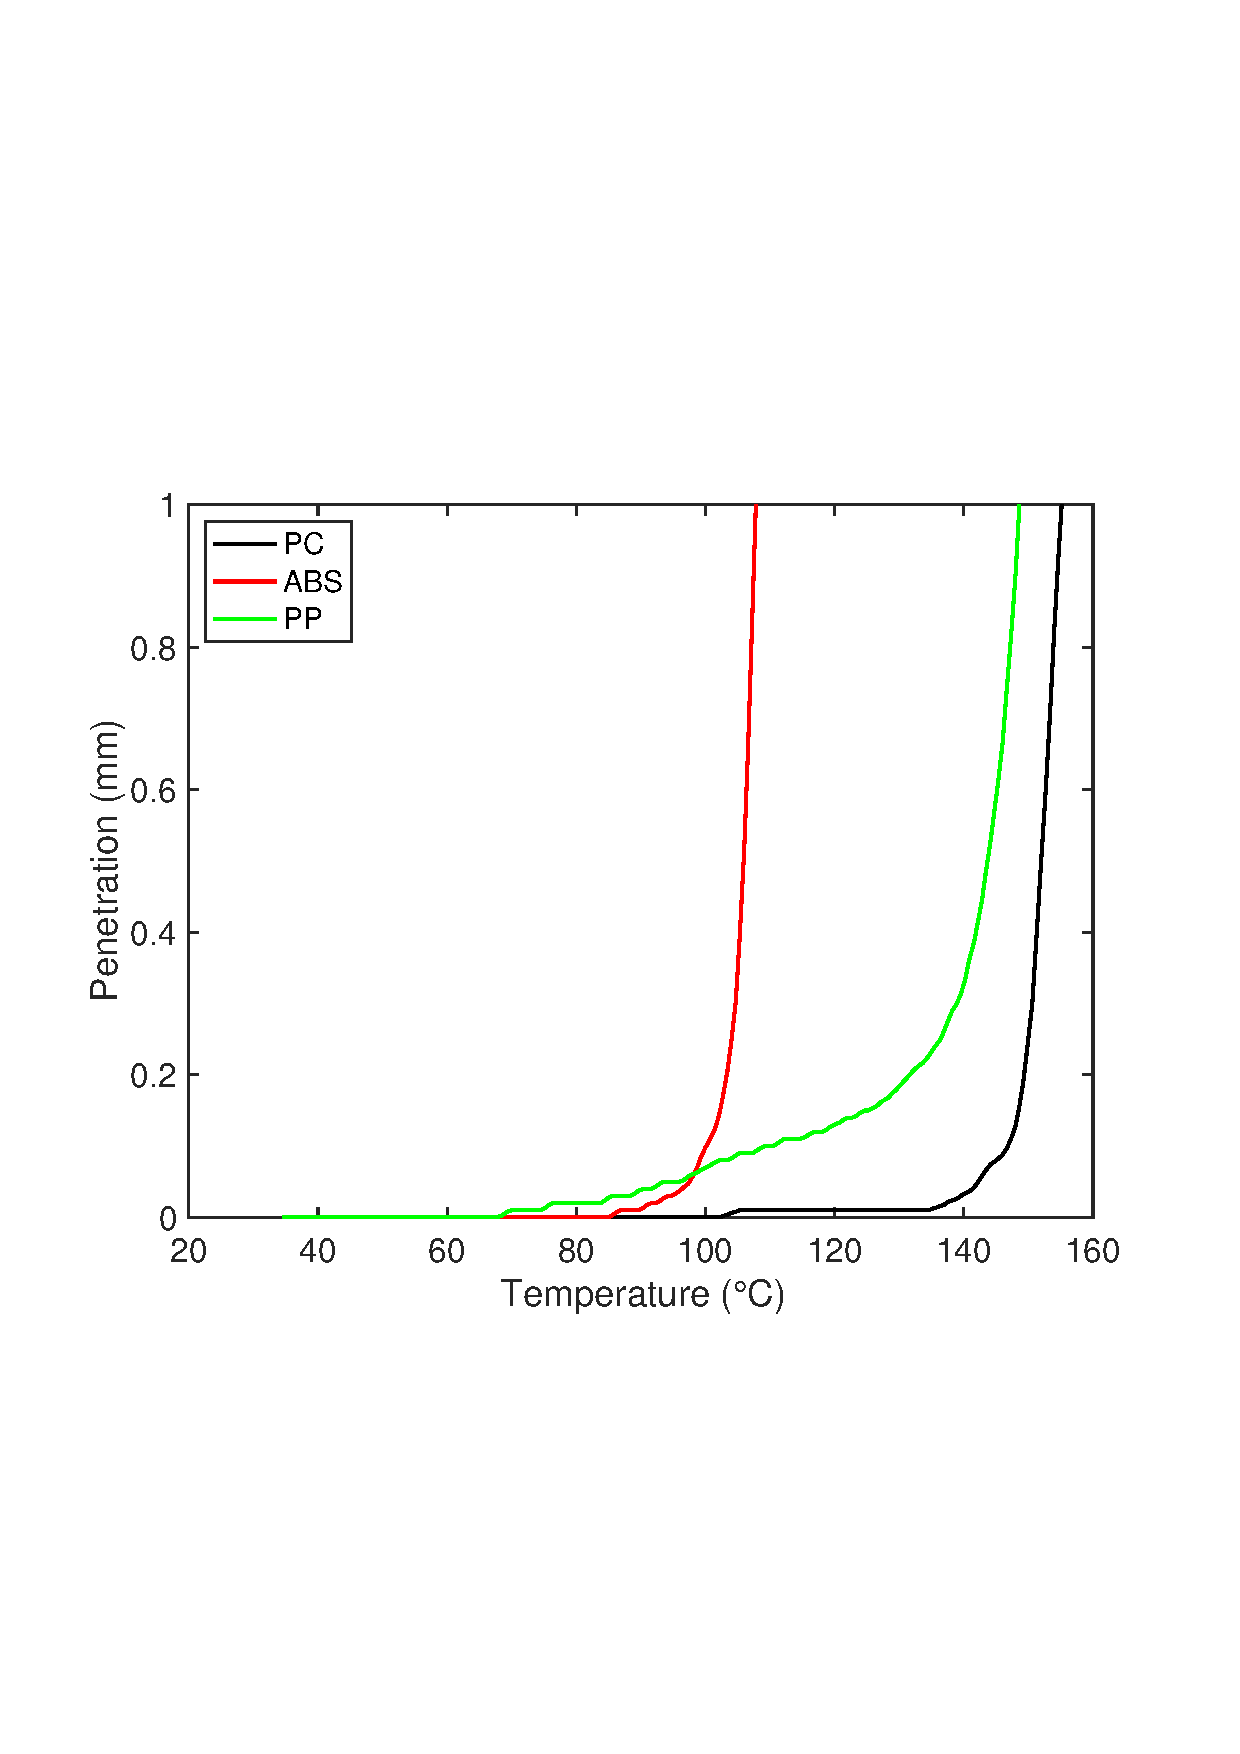
\includegraphics[scale=0.36]{vicat10}}\qquad
	\subfloat[][]
	{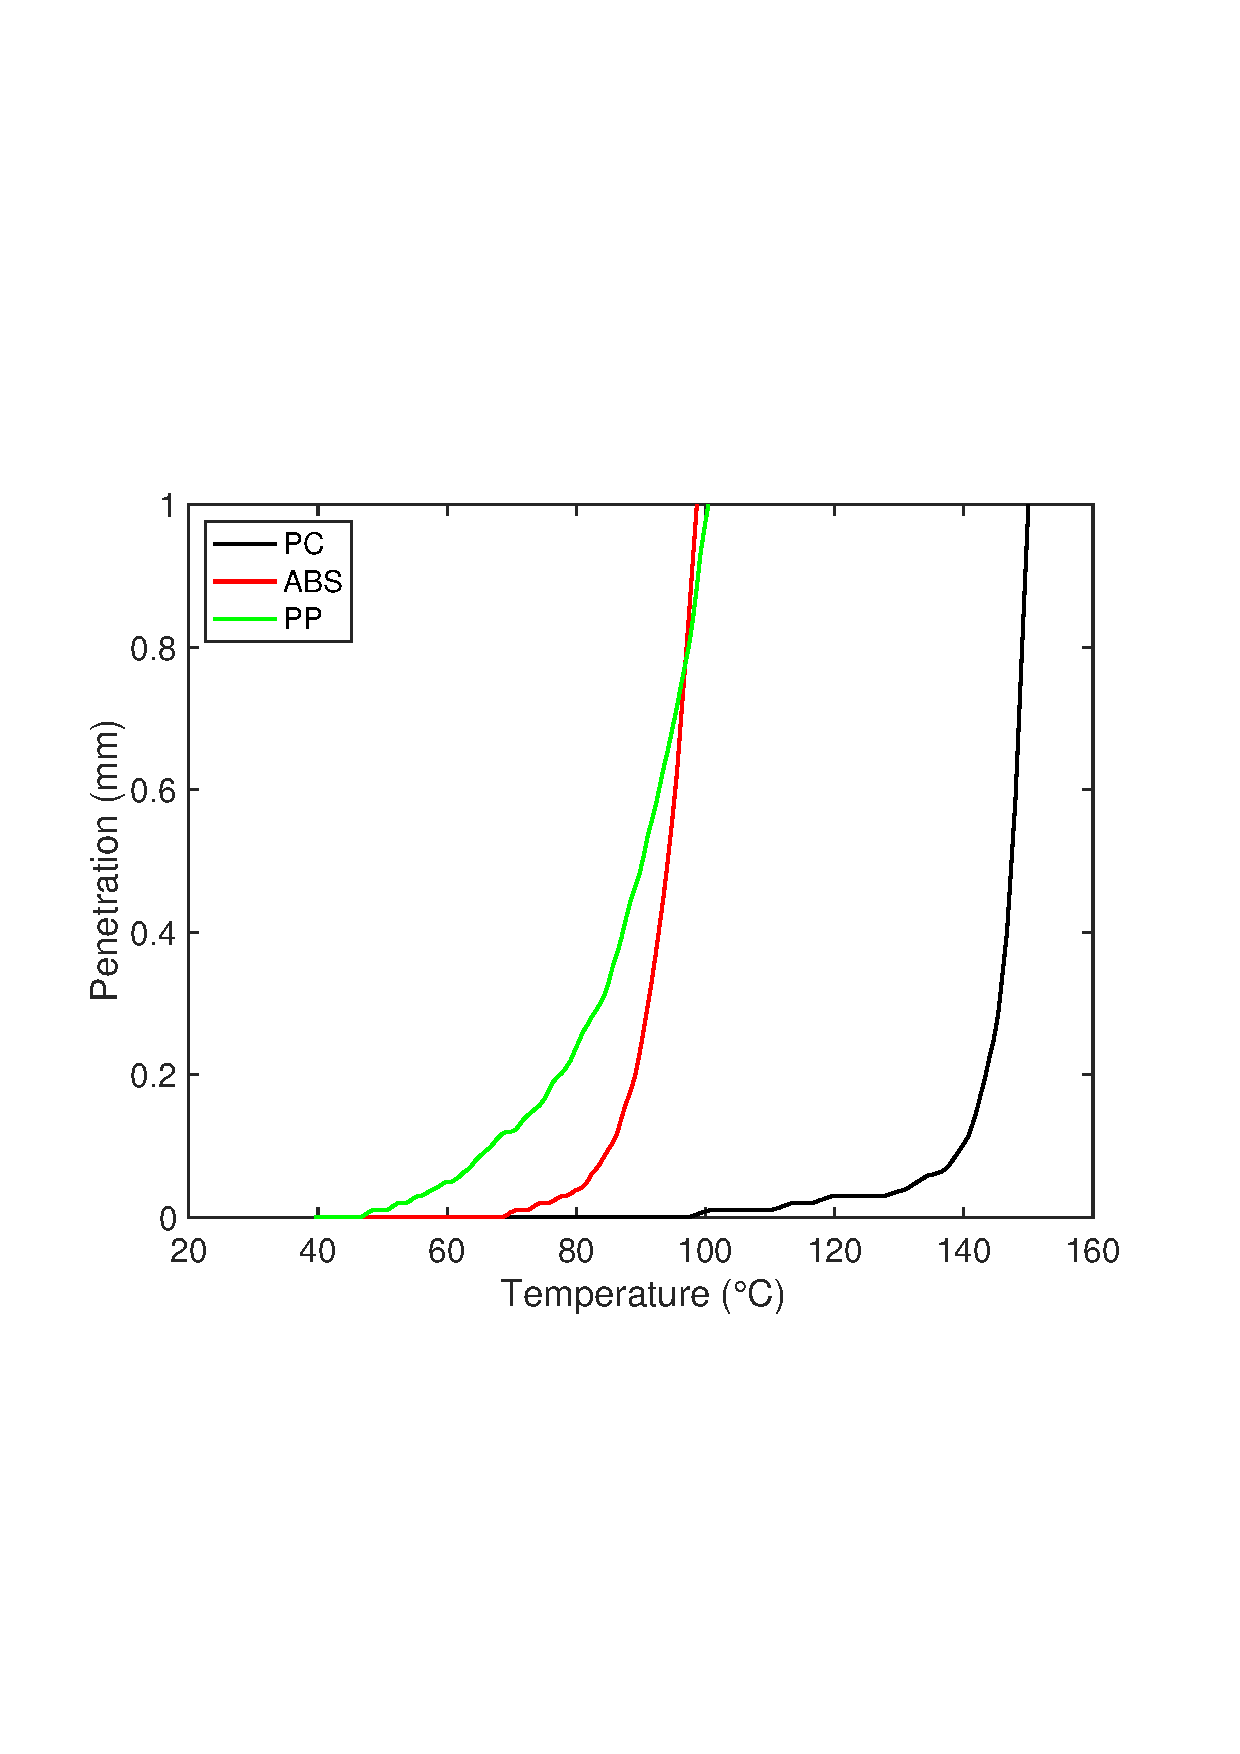
\includegraphics[scale=0.36]{vicat50}}\qquad
	\captionsetup{justification=centering}
	\caption{Vicat curves for a) $10$ N, b) $50$ N.}
	\label{fig:vicat}
\end{figure}

Analyzing the intersection between the curves and the penetration of 1 mm the following data in Table \ref{tab:vicatt} are obtained.

\begin{table}[htp]
	\centering
	$
	\begin{array}{ccccc}
	\toprule
	\textbf{Sample} & \mathbf{T_{m}} & \mathbf{T_{g}} & \mathbf{T_{vicat}^\textbf{10}} & \mathbf{T_{vicat}^\textbf{50}} \\
	\midrule
	\text{PC} & - & 149 & 154.6 & 150.0\\
	\text{ABS} & - & 105 & 107.8 & 98.0\\
	\text{PP} & 165 & -10 & 148.6 & 99.2\\
	\bottomrule
	\end{array}
	$
	\caption{Vicat temperatures ($^\circ$C).}
	\label{tab:vicatt}
\end{table}

Since PC and ABS are amorphous polymers, their Vicat temperatures don't change substantially with the load. This is due to the fact that the Vicat temperature corresponds to the glass transition temperature $T_{g}$ at which the polymer collapses under any load.
PP instead is a semicrystalline polymer, so its Vicat temperature varies considerably with the load. This can be explained by the presence of a rubbery amorphous phase that can be easily penetrated by the indent. The higher the load, the faster is the penetration and the lower the Vicat Temperature. 
\newpage

\subsection{Melt flow index (MFI) measurement}

In Figure \ref{fig:dieswell} die swell measurements for PP-1 sample in function of pressure and temperature are reported.
\begin{figure}[h!]
	\centering
	\subfloat[][]
	{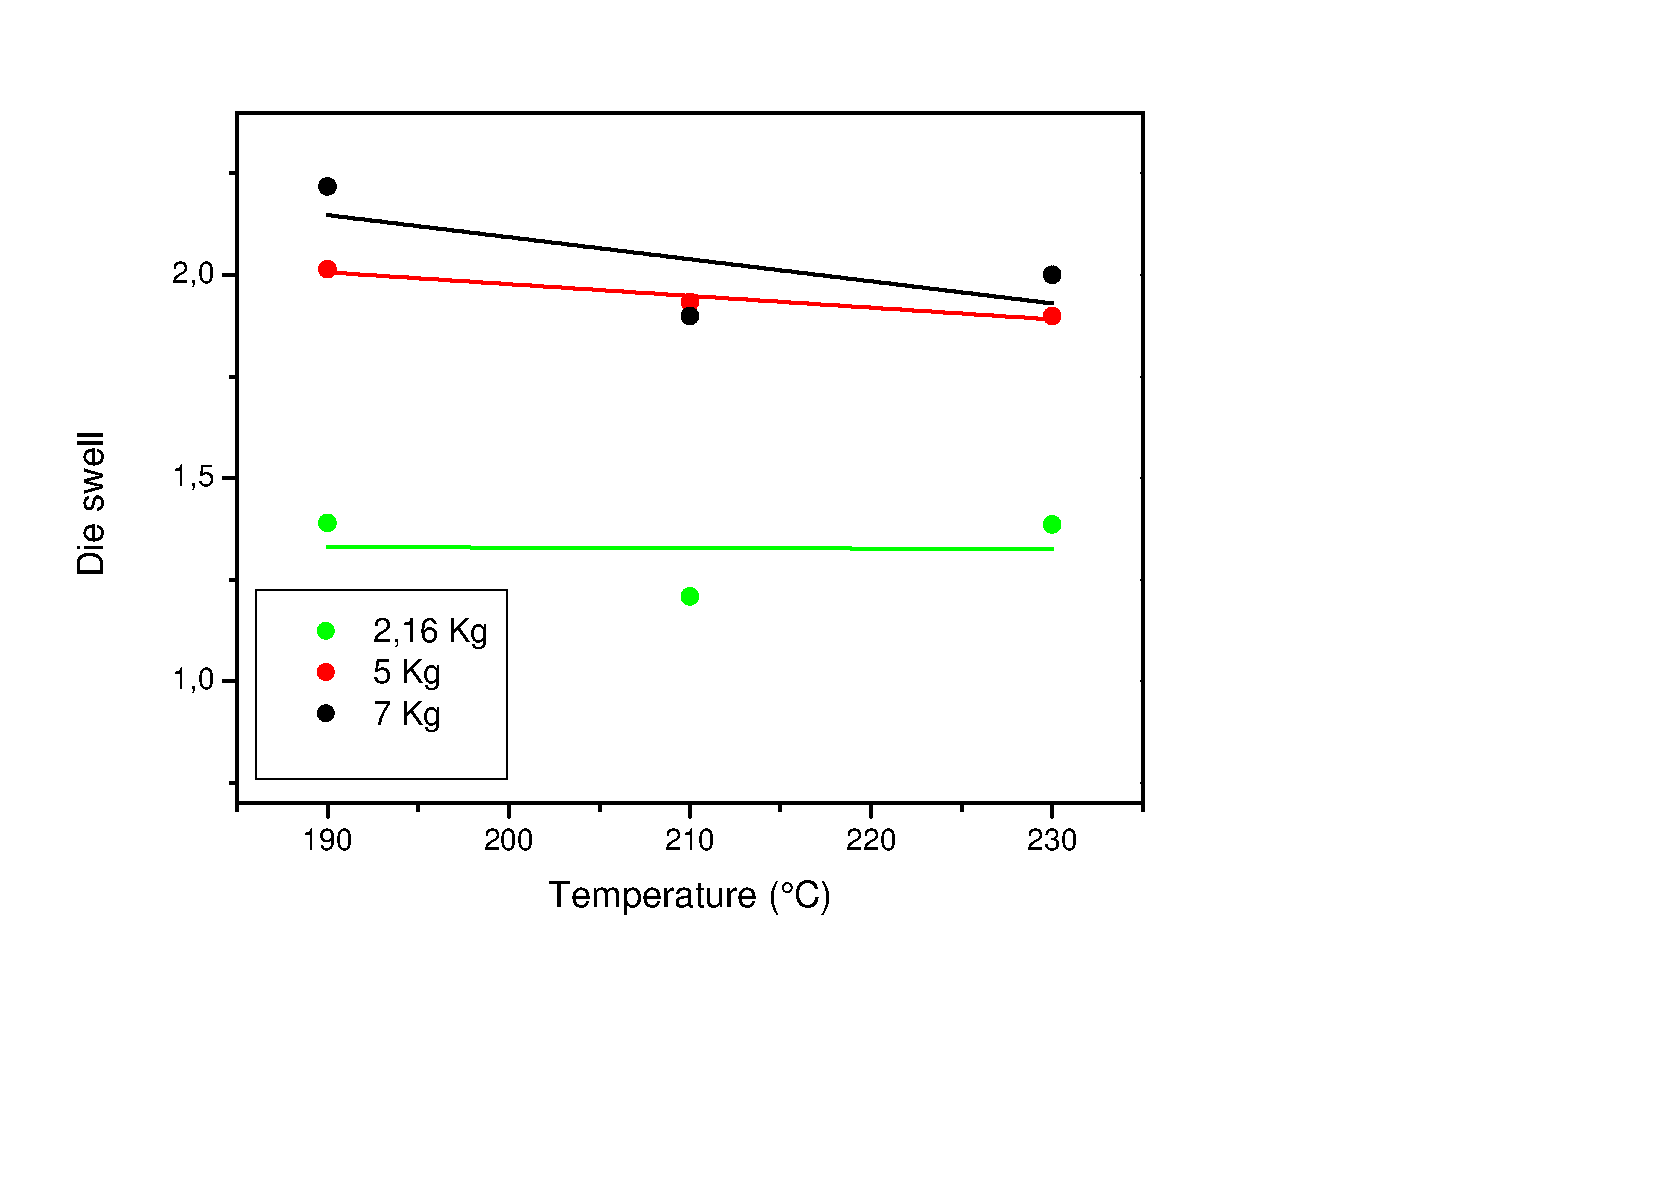
\includegraphics[scale=0.29]{dieswell}} \quad 
	\subfloat[][]
	{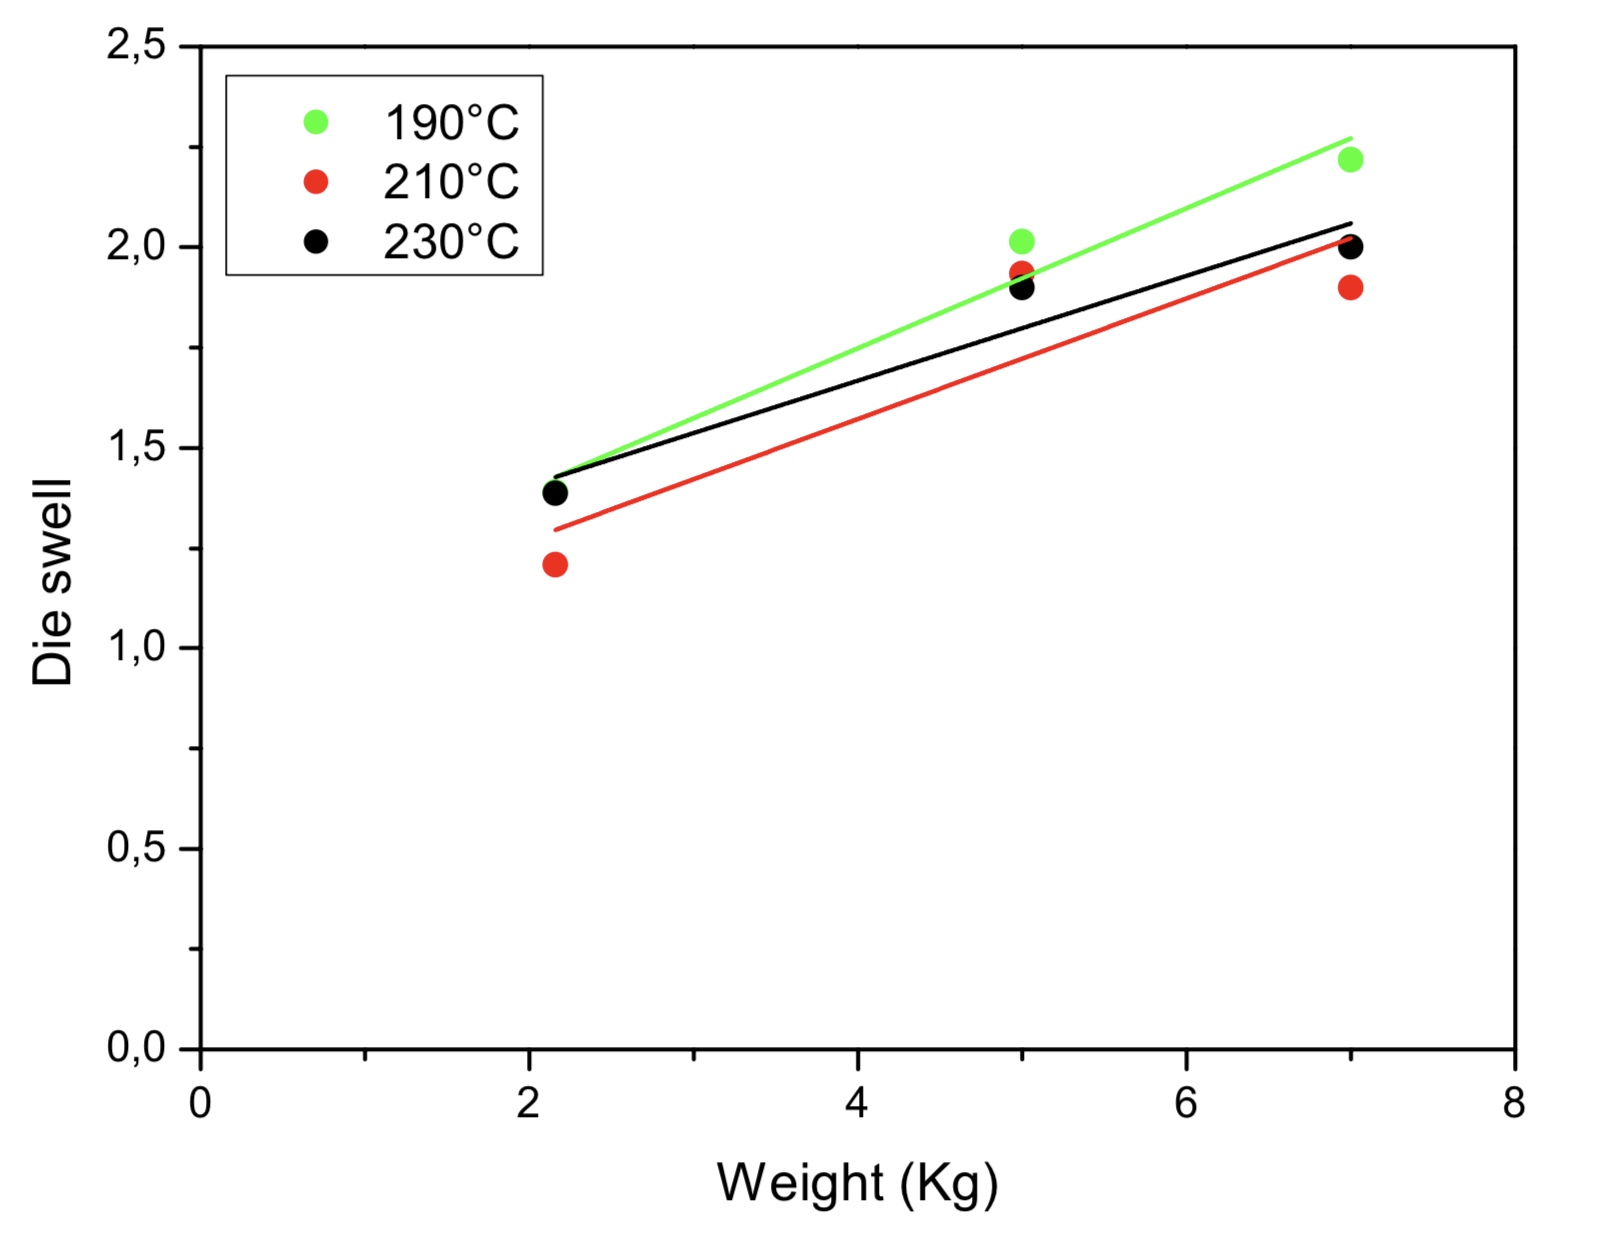
\includegraphics[scale=0.29]{dieswell2}}
	\captionsetup{justification=centering}
	\caption{Die swelling for PP–1 sample.}
	\label{fig:dieswell}
\end{figure}\\
From Figure \ref{fig:dieswell} it can be noticed that die swell increases with the applied load. This can be explained by the fact that higher loads means higher pressures and consequently, when the material exits from the die, it will present a higher relaxation of tensions thus a higher die swelling. Moreover it can be observed that die swell is not affected by the increment of temperature. The experimental data in figure \ref{fig:dieswell} follow a linear behaviour and the intercepts from the regression lines give us the value of the die swell without any load applied. These values can be related to the effect of temperature on swelling.
In Table \ref{tab:dieswell1} the values of intercepts and slopes with their standard deviations are reported.
\begin{table}[htp]
	\centering
	$
	\begin{array}{ccc}
	\toprule
	\textbf{Temperature}\, (^\circ \text{C}) & \textbf{Intercept} & \textbf{Slope} \, (1/^\circ \text{C}) \\
	\midrule
	190 & 1.05 \pm 0.17 & 0.17 \pm 0.03 \\
	210 & 0.97 \pm 0.39 & 0.15 \pm 0.08 \\
	230 & 1.15 \pm 0.18 & 0.13 \pm 0.04 \\
	\bottomrule
	\end{array}
	$
	\caption{Die swelling, results of interpolation.}
	\label{tab:dieswell1}
\end{table}\\
It is known that a rise in temperature can increase the rate of stress relaxation, leading to a decrease in extrudate swell. Moreover, a reduction of viscosity caused by an increase in temperature contributes to a decrease in extrudate swell, because of a reduction in stress applied to polymer molecules.
Therefore, there is a competition between these two effects; in fact, an increase in applied load decreases the die swell while increasing the temperature, the swell reduces.~\cite{swell}
\newpage
In Figure \ref{fig:mfi} melt flow index chart in function of temperature and parametric with pressure for PP–1 sample is reported. Standard deviations are not reported since they are too small (view Appendix A for raw data and standard deviations).
\begin{figure}[h!]
	\centering
	\subfloat[][]
	{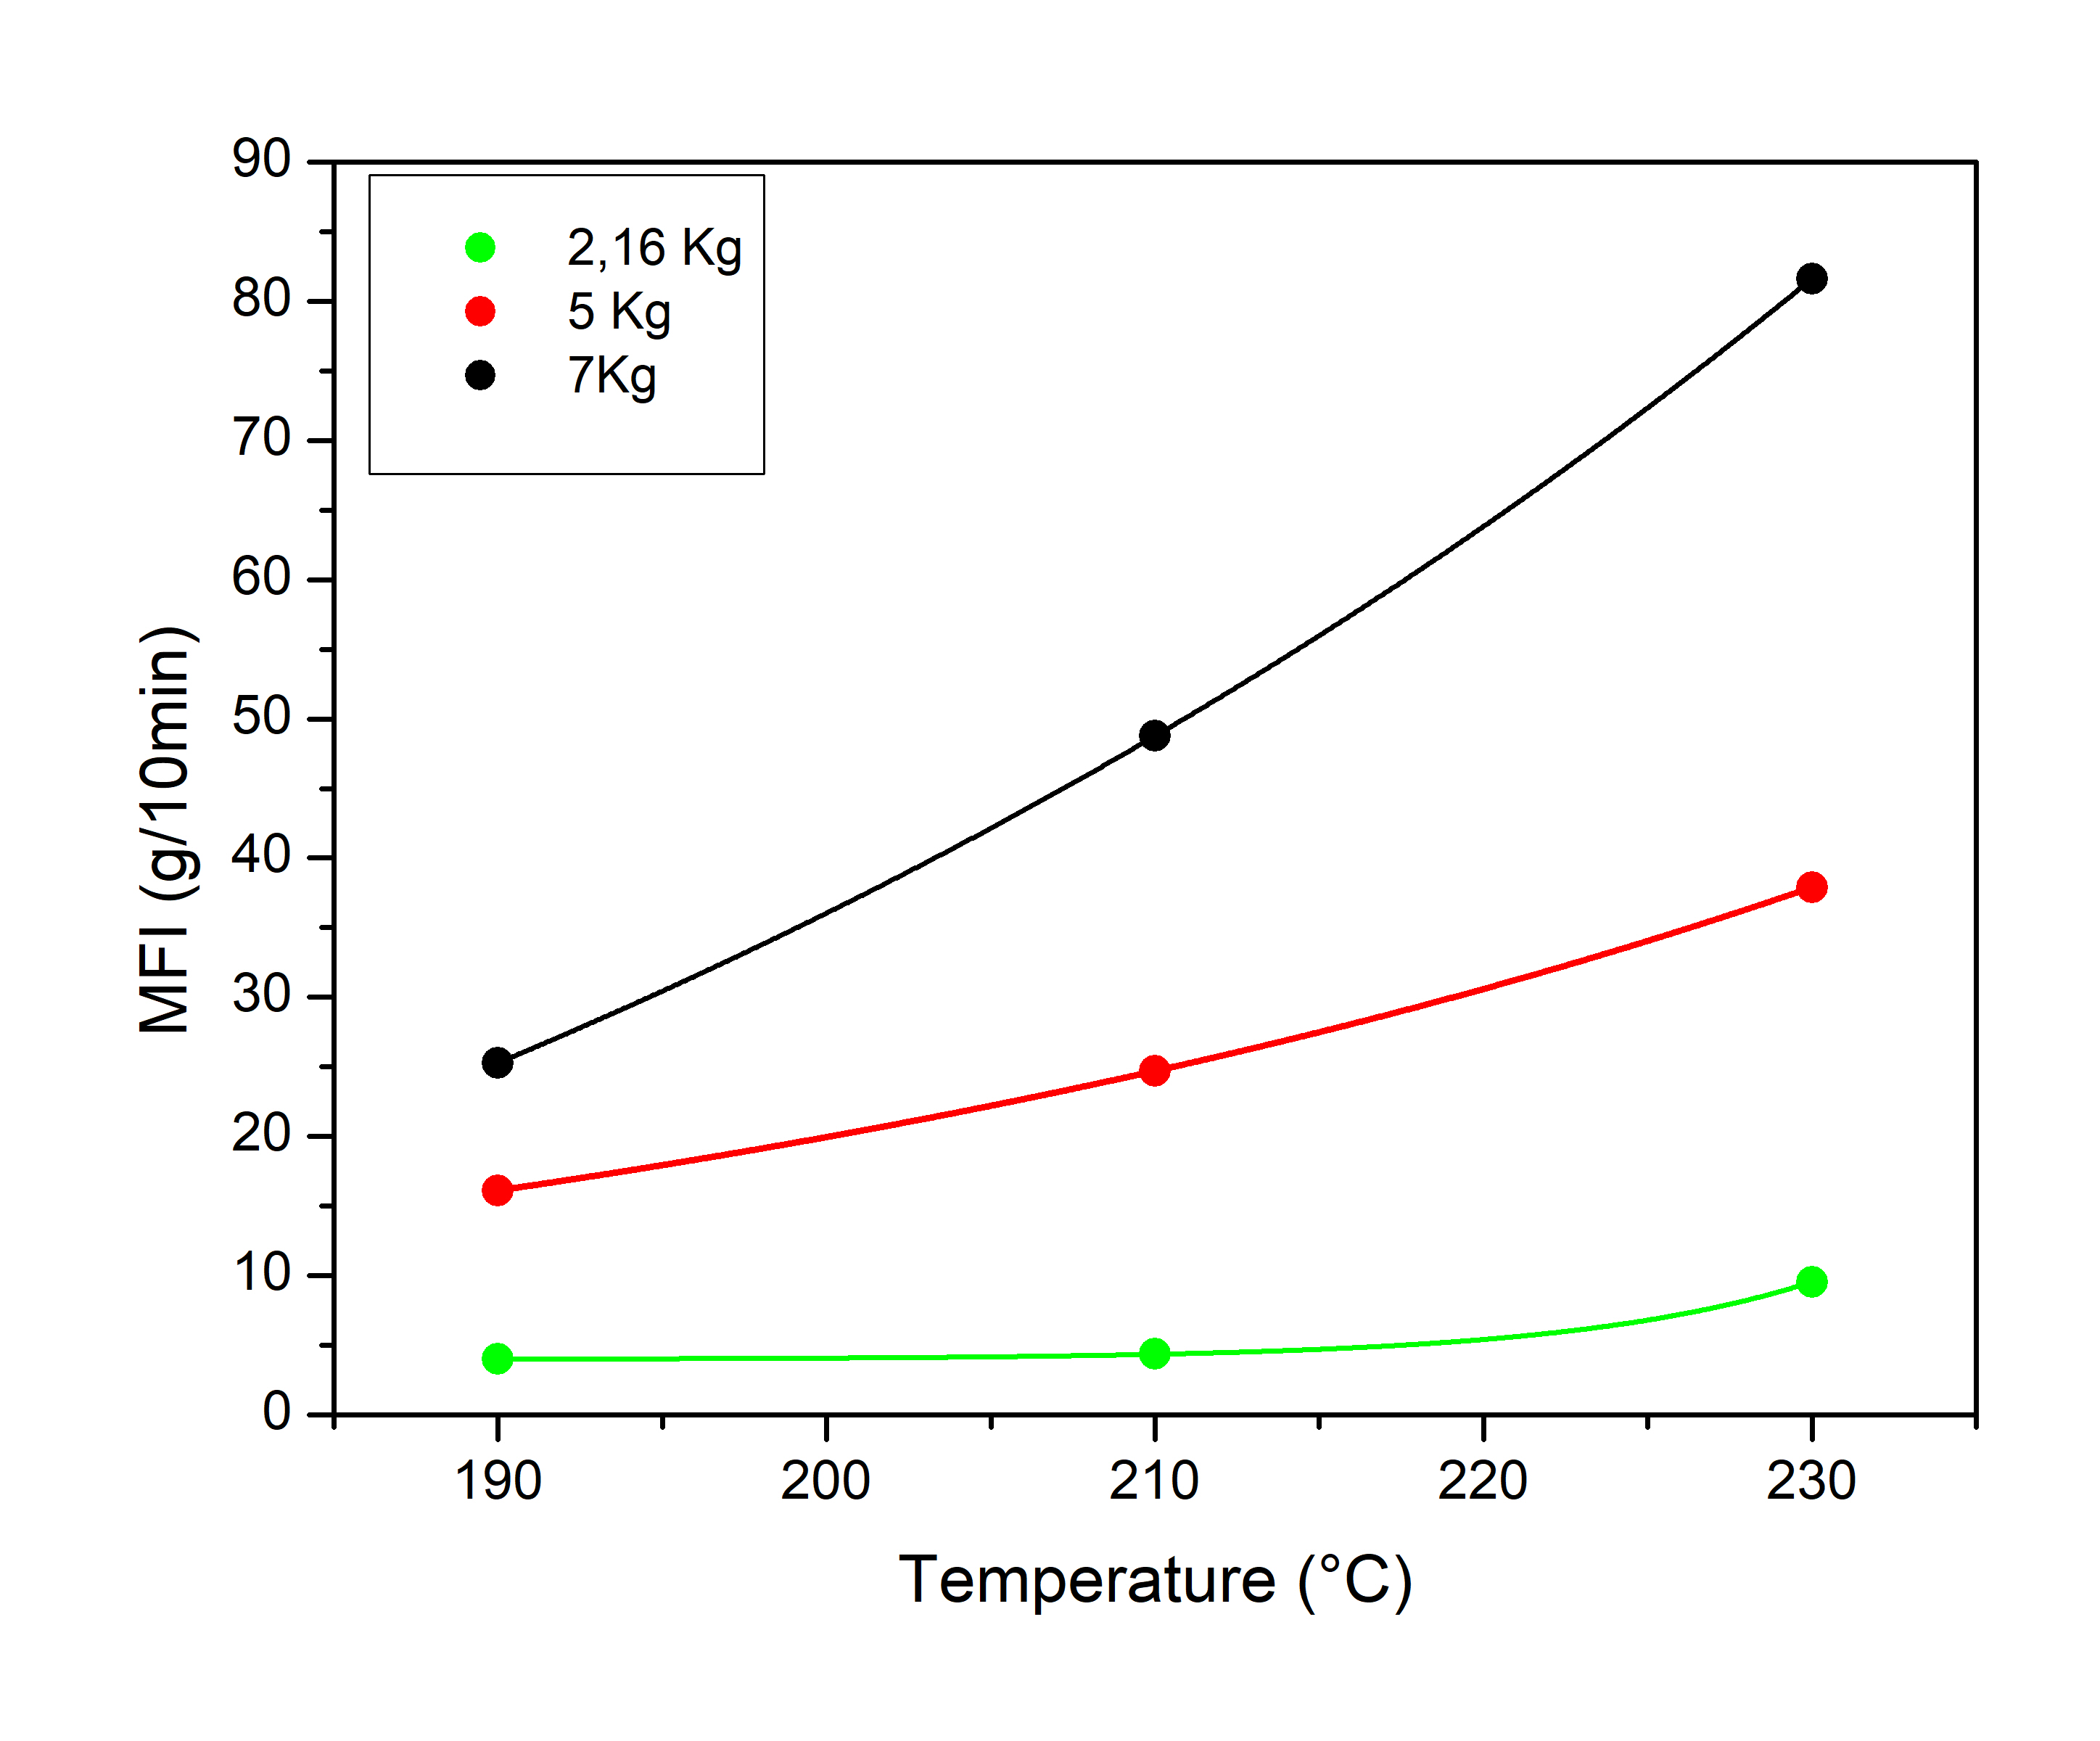
\includegraphics[scale=0.3]{mfimod}} \quad
	\subfloat[][]
	{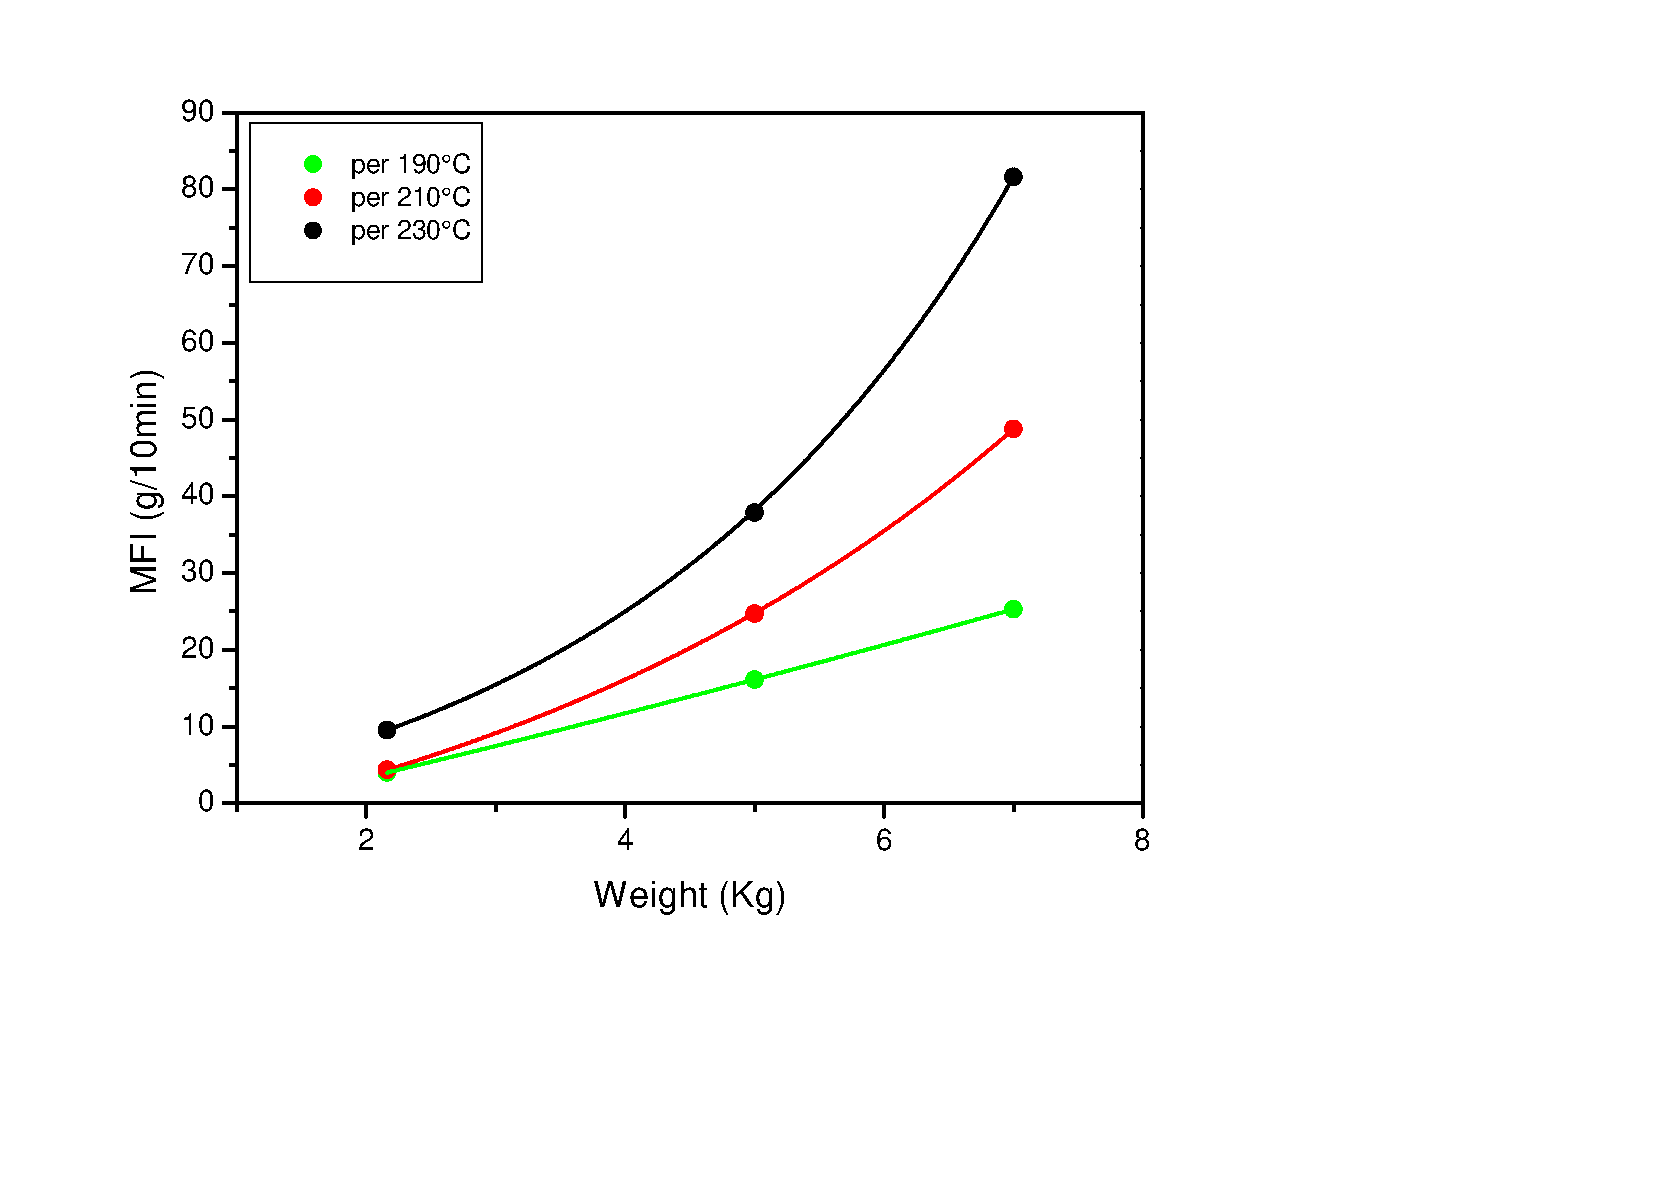
\includegraphics[scale=0.4]{mfi2}}
	\captionsetup{justification=centering}
	\caption{Melt flow index for PP–1 sample.}
	\label{fig:mfi}
\end{figure}\\
Figure \ref{fig:mfi} shows that MFI increases exponentially with temperature. This behaviour is due to the decrease of viscosity at higher temperature and thus a better flowability of the material. It can be noticed that increasing the applied load the melt flow index increases exponentially due to higher applied pressures.

\newpage

\subsubsection{Molecular weight calculation}

In Figure \ref{fig:mw} the dependency of molecular weight in function of the MFI is reported.
\begin{figure}[h!]
	\centering
	{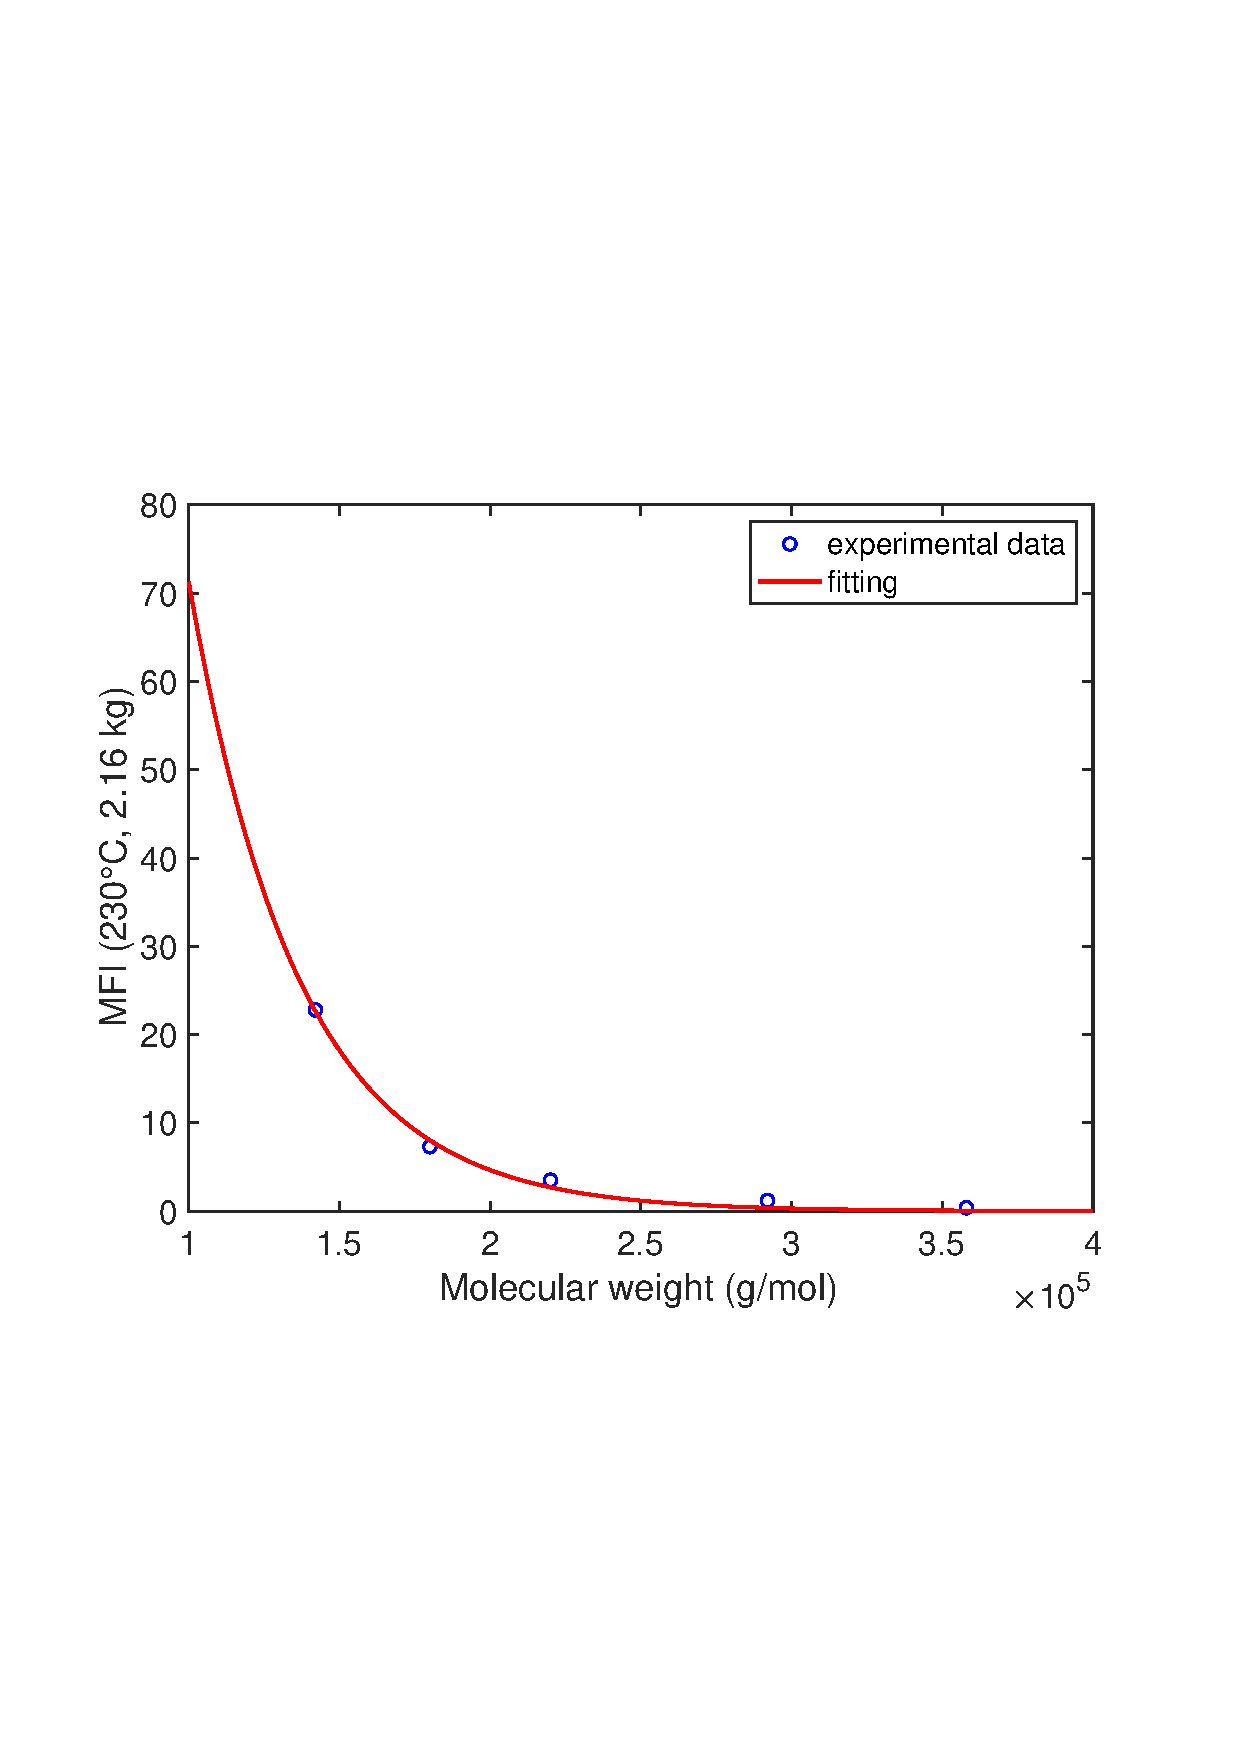
\includegraphics[scale=0.4]{mw}}
	\captionsetup{justification=centering}
	\caption{Dependency of molecular weight and MFI for polypropylene.}
	\label{fig:mw}
\end{figure}\\
The Figure \ref{fig:mw} shows that increasing MFI the molecular weight decreases exponentially. From interpolation the resulting expression is reported in Equation \ref{eq:mw}. 
\begin{equation}
\text{MFI} = 1091\cdot \exp({-2.729\cdot 10^{-05}\cdot\text{MW}})
\label{eq:mw}
\end{equation}
In Table \ref{tab:mw} the values of MFI and molecular weight are reported for the three types of PP evaluted at $230 ^\circ$C under $2.16$ \text{kg}.
\begin{table}[htp]
\centering
$
\begin{array}{lccc}
\toprule
\text{} & \textbf{PP–1} & \textbf{PP–2} & \textbf{PP–3} \\
\midrule
\text{MFI (g/10min)} & 9.56 & 1.72 & 22.75  \\
\text{MW (g/mol)}\cdot 10^{-5} & 1.74 & 2.36 & 1.42 \\
\bottomrule
\end{array}
$
\caption{MFI and MW values of the three types of PP at 230°C and 2.16Kg}
\label{tab:mw}
\end{table}\\
The molecular weight influences also the die swell. In Table \ref{tab:dieswell} the die swell values of the three types of PP evaluted at $230 ^\circ$C under $2.16$ \text{kg} are reported.
\begin{table}[htp]
\centering
$
\begin{array}{cccc}
\toprule
\text{} & \textbf{PP-1} & \textbf{PP-2} & \textbf{PP-3} \\
\midrule
\text{Die swell} & 1.39 & 1.26 & 2.47  \\
\bottomrule
\end{array}
$
\caption{Die swell values of three types of PPs. See raw data in Appendix B}
\label{tab:dieswell}
\end{table}\\
It can be seen that the higher the molecular weight the lower die swell values. High molecular weight means longer chains and this leads to high possibility of orientation and consequently a less expansion of diameter at the die exit.

\newpage

\subsubsection{Activation energy calculation}

In the following Figure \ref{fig:arrhenius} the chart of MFI measurements (Arrhenius plot) is reported, in function of temperature and applied pressure. 
\begin{figure}[h!]
	\centering
	{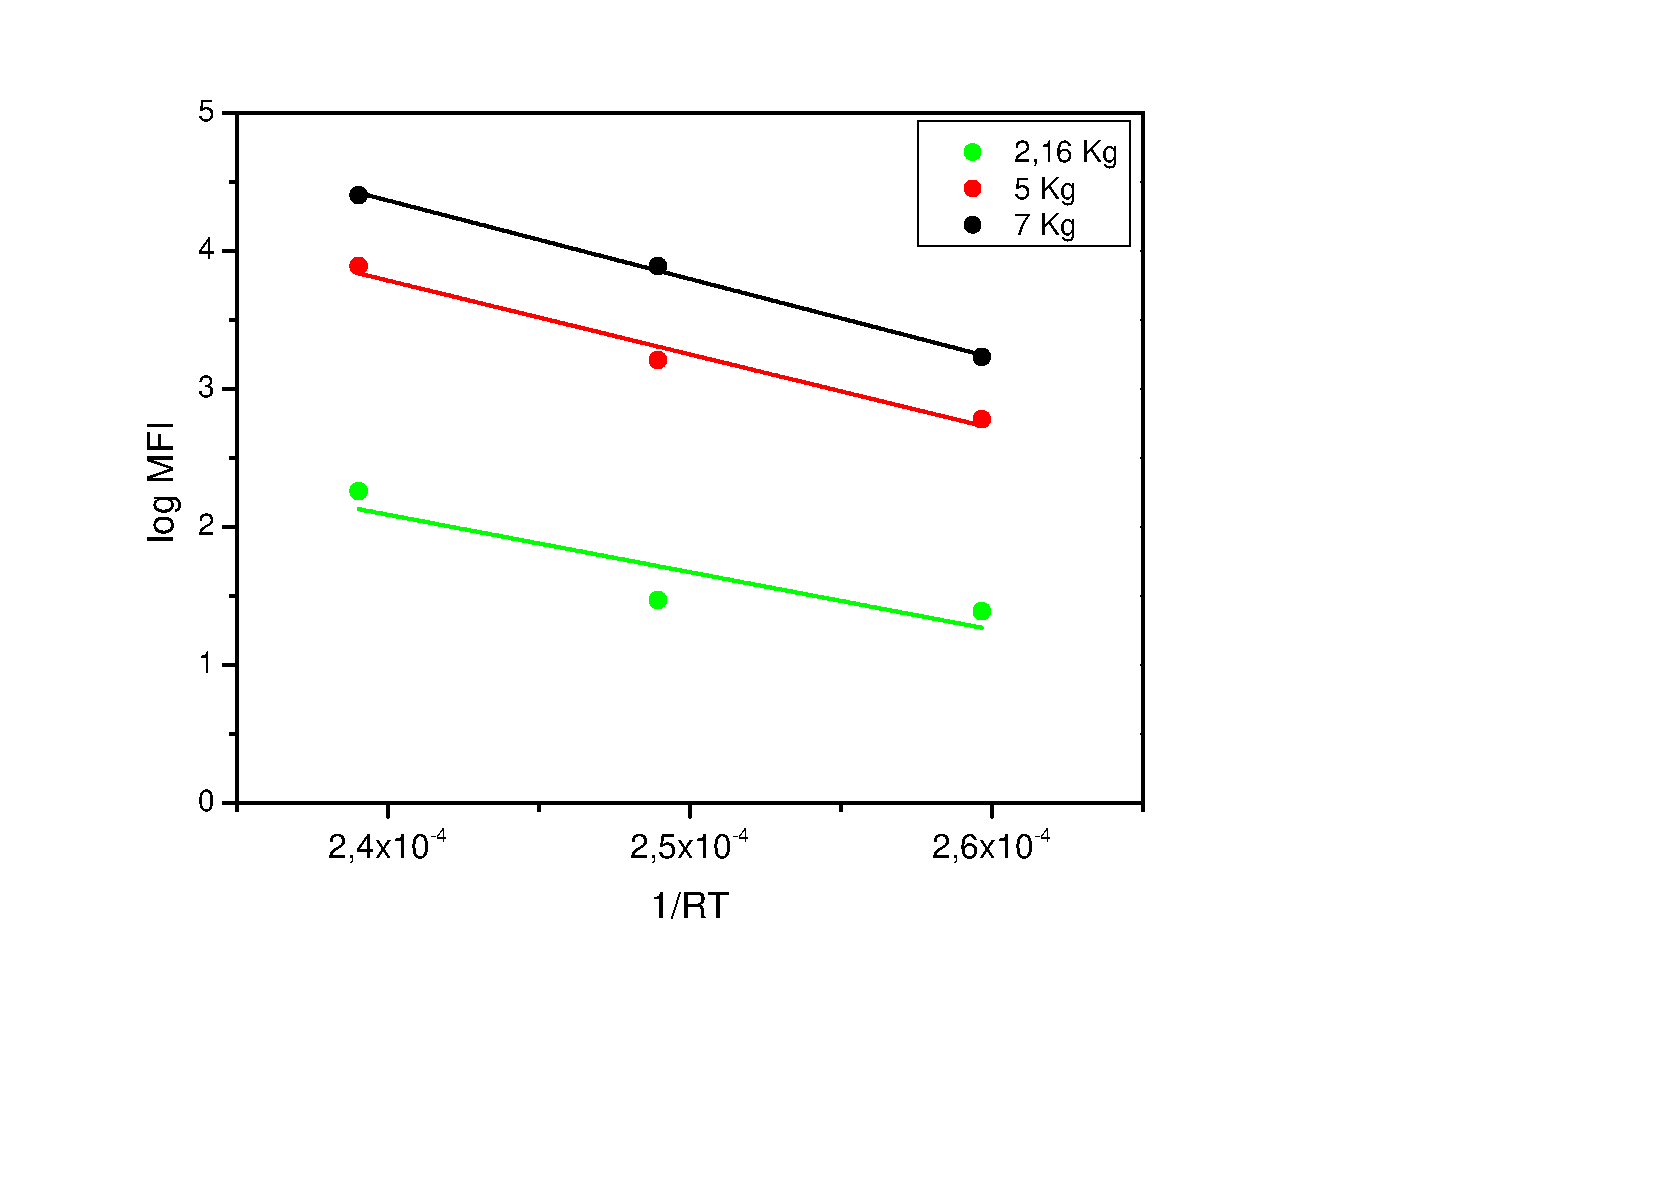
\includegraphics[scale=0.4]{arrhenius}}
	\captionsetup{justification=centering}
	\caption{MFI chart (Arrhenius plot) for PP–1 sample.}
	\label{fig:arrhenius}
\end{figure}\\
Figure \ref{fig:arrhenius} shows the relation between the MFI and the reciprocal of the temperature. In Table \ref{tab:energy} the values of activation energy of PP-1 are reported.
\begin{table}[htp]
\centering
$
\begin{array}{lc}
\toprule
\textbf{Loads} & \textbf{Activation energy} \, \text{(kJ/mol)}  \\
\midrule
\text{2.16 kg} & 41.5 \pm 20.6  \\
\text{5 kg} & 53.4 \pm 8.3 \\
\text{7.06 kg} & 56.8 \pm 2.6  \\
\midrule
\text{Average} & 50.6 \pm 6.5 \\
\bottomrule
\end{array}
$
\caption{Activation energy for PP-1.}
\label{tab:energy}
\end{table}

\subsection{Shore hardness measurement}

The results of the experiment are reported in Figure \ref{fig:duro}:

\begin{figure}[htp]
	\centering
	{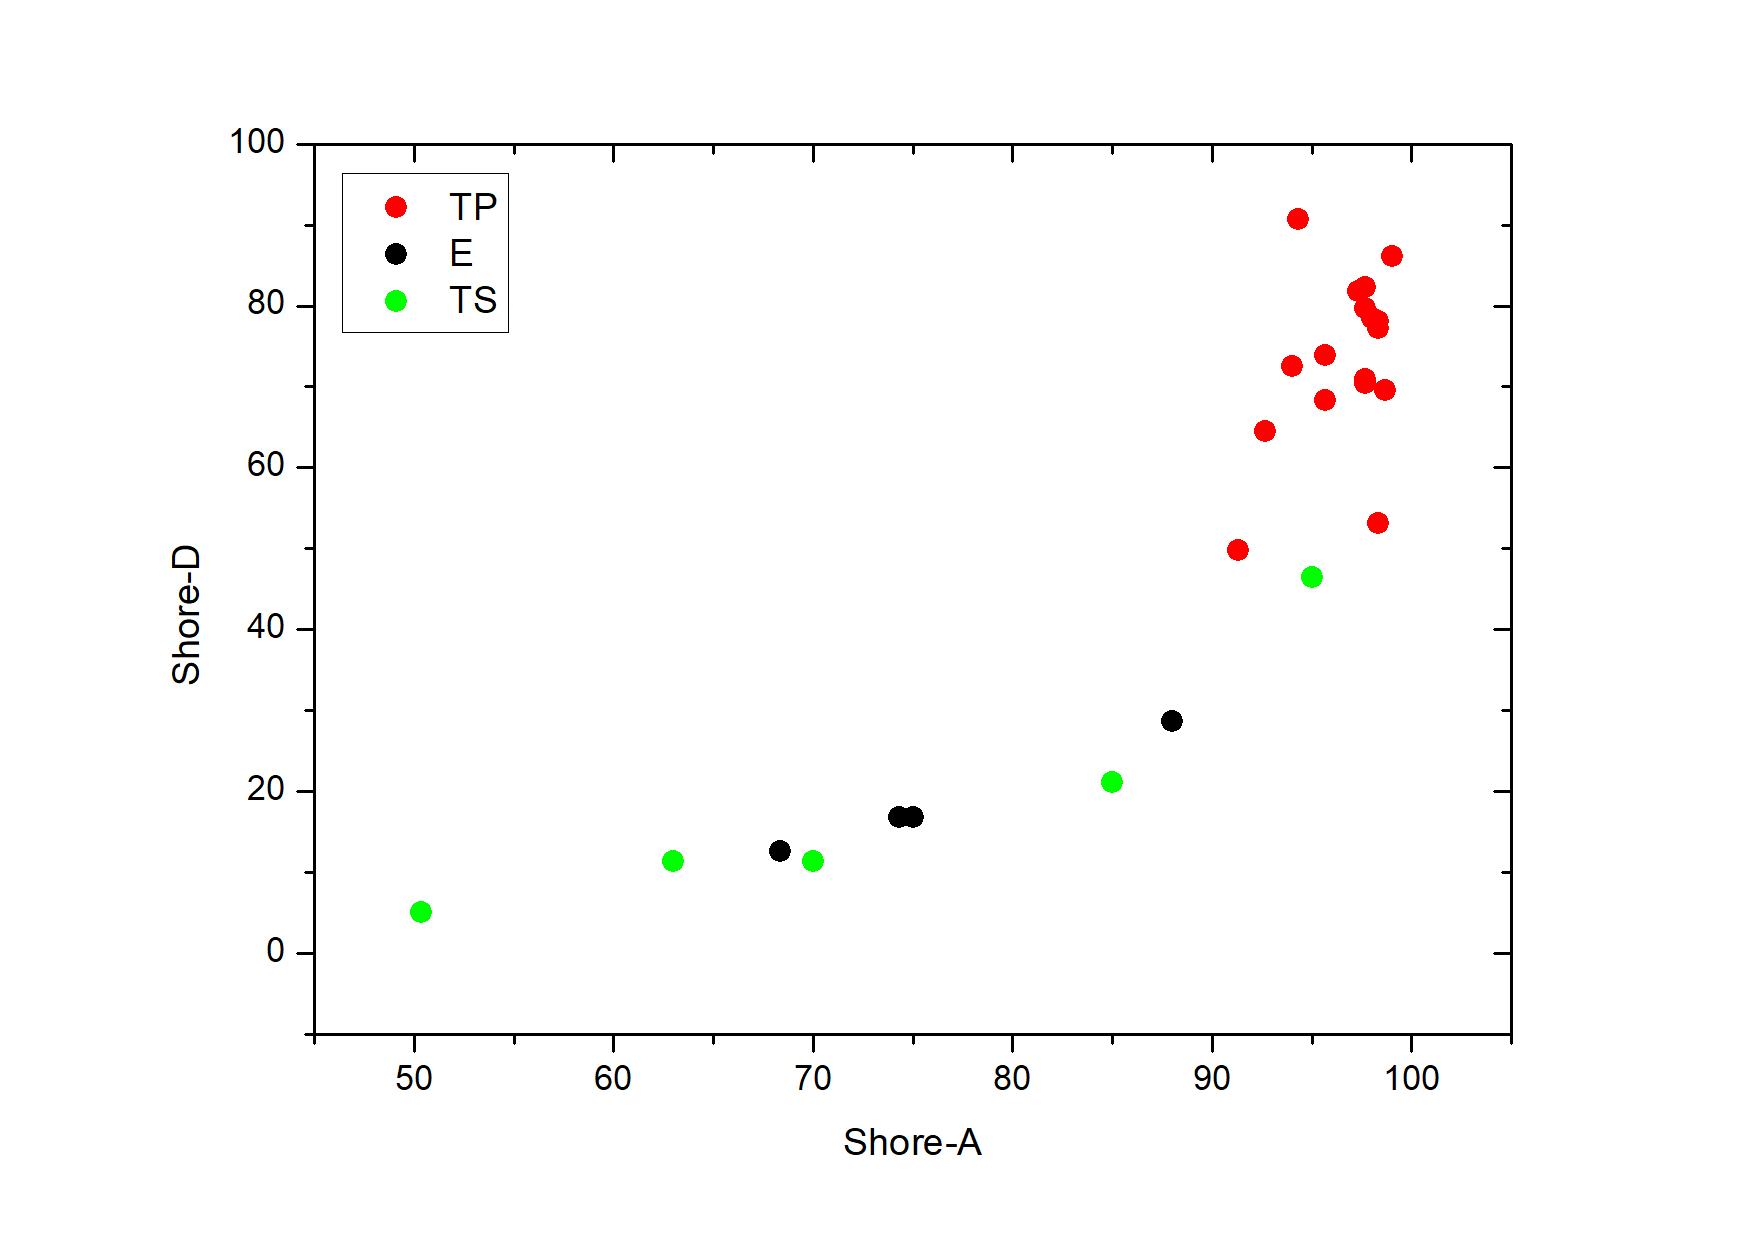
\includegraphics[scale=0.3]{duro}}
	\captionsetup{justification=centering}
	\caption{Hardness values comparison. For raw data see Appendix C.}
	\label{fig:duro}
\end{figure}

From the Figure \ref{fig:duro} it is possible to recognize the different families of polymers (thermoplastic, elastomer, thermoset). Thermoplastic polymers show the highest hardness and it is possible to verify that Shore-A is more suitable for soft materials, while Shore-D for hard ones. In fact, Shore-D shows a limited dispersion of results in respect of Shore-A for materials with lower hardness. The only thermoset polymer analized was polyurethane (PU): its particular characteristic is to have a wide range of hardness (Shore-A), from 50 to 95.

\subsection{Limit oxygen index (LOI) measurement} 

The following Table \ref{tab:loi} reports the main results obtained by this test.
\begin{table}[htp]
	\centering
	$
	\begin{array}{cclll}
	\toprule
	\textbf{Sample} & \textbf{Oxygen ($\%$)} & \textbf{Flame} & \textbf{Smoke} & \textbf{Behaviour} \\
	\midrule
	\textbf{PE} & 20 & \text{yellow} & \text{no} & \text{drips}\\
	\textbf{PP} & 22 & \text{yellow} & \text{no} & \text{drips}\\
	\textbf{PC} & 33 & \text{undefined} & \text{yes} & \text{burns}\\
	\textbf{ABS} & 20 & \text{yellow, powerful} & \text{yes, with soot} & \text{burns}\\
	\bottomrule
	\end{array}
	$
	\caption{LOI results.}
	\label{tab:loi}
\end{table}

PC sample reacts with a higher amount of flushed oxygen, meaning that this polymer is less flammable than the others.
 
\section{Conclusions}

There are many different techniques useful to analyse different polymer properties. In this laboratory session Vicat test, Shore hardness, LOI and MFI were used to investigate thermal evolution of stiffness, hardness, flammability and some rheological properties of given polymers.
Vicat temperature for amorphous polymers (like PC and ABS) corresponds to glass transition temperature at which the polymer collapses under any load; but, for semi crystalline polymers (like PP) the Vicat temperature varies with the load due to the rubbery amorphous phase which can be easily penetrated by the indent.
The melt flow index is a parameter which defines polymers ability to flow under certain conditions of load and temperature, therefore, some rheological reckonings are possible by MFI measurements. Increasing the temperature and the applied load, the MFI increases exponentially due to a decrease of viscosity. Since the MFI follows an Arrhenius-like dependence with the temperature, it is also possible to estimate the activation energy of viscous flow. Molecular weight is related to MFI: for high values MFI, the MW decreases exponentially like Mark–Houwink–Sakurada equation predicts. Moreover, die swelling is a common phenomenon in MFI and experimental data show that it has been influenced by applied load, temperature and molecular weight.
The Shore A and Shore D techniques are used to perform hardness tests on polymer samples: the first one is suitable for softer materials while the second one is suitable for the harder ones.
The LOI is the minimum oxygen percentage needed to ignite a polymer bar which will have to maintain the flame for at least 3 minutes. This percentage is then used to compare polymer flammability.

\newpage

\thispagestyle{empty}

\begin{thebibliography}{1}

\bibitem{handbook} Polymer handbook, J. Brandrup, E.H. Immergut, third edition, New York, Wiley \& Sons 2003.
\bibitem{MFI} ASTM D1238–10 “Melt flow rates of thermoplastics by extrusion”. 
\bibitem{LOI} ASTM D2863–06a “Standard test method for measuring the minimum oxygen concentration to support candle-like combustion of plastics”.
\bibitem{VICAT} ASTM D1525 “Standard test method for Vicat softening temperature of plastics”
\bibitem{SHORE} ASTM D2240 Type A and Type D “Standard test method for rubber property”
\bibitem{swell} A review of extrudate swell in polymers - C. Sirisinha – J.Sci.Soc.Thailand 23-259-280

\end{thebibliography}

\newpage

\begin{appendices}

\section{Melt flow index}

\begin{table}[htp]
	\centering
	$
	\begin{array}{ccccc}
	\toprule
	\textbf{m} \, (kg) & \textbf{t} \, (s) & \textbf{T} \, (^\circ\text{C}) & \textbf{mass} \, (g) & \textbf{diameter} \, (mm) \\ 
	\midrule
	2 & 60 & 190 & 0.3763 & 2.43 \\
	2 & 60 & 190 & 0.3761 & 2.58 \\
	2 & 60 & 190 & 0.4093 & 2.4 \\
	2 & 60 & 190 & 0.4096 &  \\ 
	2 & 60 & 190 & 0.4346 &  \\ \hline
	5 & 30 & 190 & 0.752 & 3.1 \\
	5 & 30 & 190 & 0.7892 & 2.85 \\
	5 & 30 & 190 & 0.7717 & 2.97 \\
	5 & 30 & 190 & 0.8279 &  \\
	5 & 30 & 190 & 0.8912 &  \\ \hline
	7 & 15 & 190 & 0.6683 & 3.28 \\
	7 & 15 & 190 & 0.5827 & 3.02 \\
	7 & 15 & 190 & 0.61 & 3.06 \\
	7 & 15 & 190 & 0.6311 &  \\
	7 & 15 & 190 & 0.6693 &  \\ \hline
	2 & 30 & 210 & 0.1979 & 2.09 \\
	2 & 30 & 210 & 0.1958 & 2.46 \\
	2 & 30 & 210 & 0.1929 & 2.36 \\
	2 & 30 & 210 & 0.2194 &  \\
	2 & 30 & 210 & 0.2829 &  \\ \hline
	5 & 15 & 210 & 0.6135 & 2.93 \\
	5 & 15 & 210 & 0.599 & 2.97 \\
	5 & 15 & 210 & 0.6112 & 2.84 \\
	5 & 15 & 210 & 0.6266 &  \\ 
	5 & 15 & 210 & 0.6380 &  \\ \hline
	7 & 10 & 210 & 0.8135 & 2.86 \\ 
	7 & 10 & 210 & 0.8102 & 3.01 \\ 
	7 & 10 & 210 & 0.815 & 2.79 \\ \hline
	2 & 10 & 230 & 0.1682 & 2.44 \\
	2 & 10 & 230 & 0.1491 & 2.6 \\ 
	2 & 10 & 230 & 0.1558 & 2.36 \\ 
	2 & 10 & 230 & 0.1523 &  \\
	2 & 10 & 230 & 0.1709 &  \\ \hline
	5 & 10 & 230 & 0.6354 & 2.89 \\
	5 & 10 & 230 & 0.6013 & 2.79 \\
	5 & 10 & 230 & 0.5948 & 2.98 \\
	5 & 10 & 230 & 0.6518 &  \\
	5 & 10 & 230 & 0.6746 &  \\ \hline
	7 & 5 & 230 & 0.8169 & 2.88 \\
	7 & 5 & 230 & 0.6869 & 3.02 \\
	7 & 5 & 230 & 0.6357 & 2.99 \\
	7 & 5 & 230 & 0.4969 &  \\
	7 & 5 & 230 & 0.7635 &  \\
	\bottomrule
\end{array}
$
	\caption{Experimental data for Melt Flow Index measurament of sample PP-1.}
	\label{tab:exmfi}
\end{table}


\begin{table}[htp]
	\centering
	$
	\begin{tabular}{c|ccc}
	\toprule
	\textbf{MFI} & 190 & 210 & 230\\
	\midrule
	2.16 & 4.01 $\pm$ 0.25 & 4.36 $\pm$ 0.76 & 9.56 $\pm$ 0.58\\
	5 & 16.13 $\pm$ 1.10 & 24.71 $\pm$ 0.60 & 37089 $\pm$ 2.02\\
	7 & 25.29 $\pm$ 1.50 & 48.77 $\pm$ 0.15 & 81.60 $\pm$ 14.85\\
	\bottomrule
	\end{tabular}
	$
	\caption{Melt flow index values and standard deviations. m (kg) vs T ($^\circ$C)}
	\label{tab:tmwpp}
\end{table}

\section{Die swell}

\begin{table}[htp]
	\centering
	$
	\begin{array}{cccc}
	\toprule
	\textbf{Sample} & \textbf{Specimen} & \textbf{Mass}\, (g) & \textbf{Diameter}\, (mm)\\
	\midrule
	 & 1 & 0.3763 & 2.43\\
	PP-1 & 2 & 0.3761 & 2.58\\
	 & 3 & 0.4093 & 2.4\\
	\midrule
	 & 1 & 0.1832 & 2.4\\
	PP-2 & 2 & 0.1643 & 2.34\\
	 & 3 & 0.1682 & 2.33\\
	\midrule
	 & 1 & 0.3689 & 3.3\\
	PP-3 & 2 & 0.3648 & 3.22\\
	 & 3 & 0.3935 & 3.36\\
	\bottomrule
	\end{array}
	$
	\caption{Experimental data for die swell calculation of three types of PPs at T = 230$^\circ$C and under a load of 2.16 kg.}
	\label{tab:tmwpp}
\end{table}

\section{Shore hardness measurement}

\begin{table}[htp]
	\centering
	$
	\begin{array}{lccccc}
	\toprule
	\textbf{Sample} & \textbf{Specimen 1} & \textbf{Specimen 2} & \textbf{Specimen 3} & \textbf{AVG} & \textbf{Proper AVG} \\
	\midrule
	1&65&64&65&65&82\\
2&65&65&64&65&82\\
3&56&55&57&56&71\\
4&38&39&41&39&50\\
5&63&63&63&63&80\\
6&65&64&66&65&82\\
7&56&58&58&57&73\\
8&13&14&13&13&17\\
9&13&13&14&13&17\\
10&61&62&63&62&78\\
11&72&71&72&72&91\\
12&25&21&22&23&29\\
13&57&59&59&58&74\\
14&16&17&17&17&21\\
15&10&11&9&10&13\\
16&56&55&56&56&70\\
17&68&68&68&68&86\\
18&9&9&9&9&11\\
19&51&51&51&51&65\\
20&36&37&37&37&46\\
21&42&42&42&42&53\\
22&62&63&60&62&78\\
23&54&54&54&54&68\\
24&55&55&55&55&70\\
25&9&10&8&9&11\\
26&61&61&61&61&77\\
27&4&4&4&4&5\\
	\bottomrule
	\end{array}
	$
	\caption{Shore-D data}
	\label{tab:shored}
\end{table}

\begin{table}[htp]
	\centering
	$
	\begin{array}{lcccc}
	\toprule
	\textbf{Sample} & \textbf{Specimen 1} & \textbf{Specimen 2} & \textbf{Specimen 3} & \textbf{AVG} \\
	\midrule
	1&98&97&97&97\\
2&96&98&98&97\\
3&98&97&98&98\\
4&92&91&91&91\\
5&98&97&98&98\\
6&98&98&97&98\\
7&94&94&94&94\\
8&74&74&75&74\\
9&74&76&75&75\\
10&98&98&98&98\\
11&97&93&93&94\\
12&85&90&89&88\\
13&97&93&97&96\\
14&85&85&85&85\\
15&68&68&69&68\\
16&97&98&98&98\\
17&99&99&99&99\\
18&64&63&62&63\\
19&92&91&95&93\\
20&95&96&94&95\\
21&98&99&98&98\\
22&98&98&99&98\\
23&97&94&96&96\\
24&99&99&98&99\\
25&70&70&70&70\\
26&99&98&98&98\\
27&51&50&50&50\\
	\bottomrule
	\end{array}
	$
	\caption{Shore-A data}
	\label{tab:shorea}
\end{table}

\end{appendices}

\end{document}
